% Format teze zasnovan je na paketu memoir
% http://tug.ctan.org/macros/latex/contrib/memoir/memman.pdf ili
% http://texdoc.net/texmf-dist/doc/latex/memoir/memman.pdf
% 
% Prilikom zadavanja klase memoir, navedenim opcijama se podešava 
% veličina slova (12pt) i jednostrano štampanje (oneside).
% Ove parametre možete menjati samo ako pravite nezvanične verzije
% mastera za privatnu upotrebu (na primer, u b5 varijanti ima smisla 
% smanjiti 
\documentclass[12pt,oneside]{memoir}

% Paket koji definiše sve specifičnosti mastera Matematičkog fakulteta
\usepackage{matfmaster}
\usepackage{enumitem}
%
% Podrazumevano pismo je ćirilica.
%   Ako koristite pdflatex, a ne xetex, sav latinički tekst na srpskom jeziku
%   treba biti okružen sa \lat{...} ili \begin{latinica}...\end{latinica}.
%
% Opicija [latinica]:
%   ako želite da pišete latiniciom, dodajte opciju "latinica" tj.
%   prethodni paket uključite pomoću: \usepackage[latinica]{matfmaster}.
%   Ako koristite pdflatex, a ne xetex, sav ćirilički tekst treba biti
%   okružen sa \cir{...} ili \begin{cirilica}...\end{cirilica}.
%
% Opcija [biblatex]:
%   ako želite da koristite reference na više jezika i umesto paketa
%   bibtex da koristite BibLaTeX/Biber, dodajte opciju "biblatex" tj.
%   prethodni paket uključite pomoću: \usepackage[biblatex]{matfmaster}
%
% Opcija [b5paper]:
%   ako želite da napravite verziju teze u manjem (b5) formatu, navedite
%   opciju "b5paper", tj. prethodni paket uključite pomoću: 
%   \usepackage[b5paper]{matfmaster}. Tada ima smisla razmisliti o promeni
%   veličine slova (izmenom opcije 12pt na 11pt u \documentclass{memoir}).
%
% Naravno, opcije je moguće kombinovati.
% Npr. \usepackage[b5paper,biblatex]{matfmaster}

% Pomoćni paket koji generiše nasumičan tekst u kojem se javljaju sva slova
% azbuke (nema potrebe koristiti ovo u pravim disertacijama)
\usepackage{pangrami}
\usepackage{amsmath}

% Datoteka sa literaturom u BibTex tj. BibLaTeX/Biber formatu
\bib{valgrind}

% Ime kandidata na srpskom jeziku (u odabranom pismu)
\autor{Aлександра Караџић}
% Naslov teze na srpskom jeziku (u odabranom pismu)
\naslov{Алат \textit{Valgrind} - имплементација конвенције \textit{FPXX} за архитектуру \textit{MIPS} }
% Godina u kojoj je teza predana komisiji
\godina{2018}
% Ime i afilijacija mentora (u odabranom pismu)
\mentor{др Милена \textsc{Вујошевић Јаничић}, доцент\\ Универзитет у Београду, Математички факултет}
% Ime i afilijacija prvog člana komisije (u odabranom pismu)
\komisijaA{др Филип \textsc{Марић}, ванредни професор\\ Универзитет у Београду, Математички факултет}
% Ime i afilijacija drugog člana komisije (u odabranom pismu)
\komisijaB{др Јелена \textsc{Граовац}, доцент\\ Универзитет у Београду, Математички факултет}
% Ime i afilijacija trećeg člana komisije (opciono)
% \komisijaC{}
% Ime i afilijacija četvrtog člana komisije (opciono)
% \komisijaD{}
% Datum odbrane (obrisati ili iskomentarisati narednu liniju ako datum odbrane nije poznat)
\datumodbrane{31. јануар 2018.}

% Apstrakt na srpskom jeziku (u odabranom pismu)
\apstr{
Програмска подршка је све присутнија, напретком технологије долази до пораста у перформансама и могућностима рачунара. Како кориснички захтеви све више расту, самим тим расте комплексност процеса развоја софтвера. Јавља се потреба за алатима који служе за детекцију и отклањање грешака, као и за анализу и прављење профила корисничких програма. Један такав алат јесте  \textit{Valgrind}.

Архитектура \textit{MIPS} је архитектура са процесором смањеног скупа наредби и једна од заступљенијих архитектура на тржишту система са уграђеним рачунаром. Конвенција \textit{FPXX} је специфична за архитектуру \textit{MIPS}. Циљ овог рада је упознавање са алатом \textit{Valgrind} и свим могућностима које нам он нуди, упознавање са специфичностима конвенције \textit{FPXX} као и имплементација ове конвенције у оквиру алата.
}

% Ključne reči na srpskom jeziku (u odabranom pismu)
\kljucnereci{\textit{Valgrind}, \textit{MIPS}, \textit{FP} регистри, конвенција \textit{FPXX}}

\begin{document}
% ==============================================================================
% Uvodni deo teze
\frontmatter
% ==============================================================================
% Naslovna strana
\naslovna
% Strana sa podacima o mentoru i članovima komisije
\komisija
% Strana sa posvetom (u odabranom pismu)
\posveta{Деди}
% Strana sa podacima o disertaciji na srpskom jeziku
\apstrakt
% Sadržaj teze
\tableofcontents*

% ==============================================================================
% Glavni deo teze
\mainmatter
% ==============================================================================

% ------------------------------------------------------------------------------
\chapter{Увод}
% ------------------------------------------------------------------------------

\indent Тражење разлога неправилног рада система може трајати поприлично дуго, поготово ако се систем састоји из десетина хиљада линија кода и десетине па и стотине операција алоцирања и деалоцирања меморије. Под овим, подразумевамо грешке које компајлер не пријављује, попут цурења меморије или коришћење неиницијализованих вредности. За неке, још сложеније, вишенитне, системе, ове грешке се могу јавити у виду неочекиваног приступа дељеним подацима, односно утркивању за приступ истим. Један од алата који помажу у откривању оваквих грешака јесте \textit{Valgrind}~\cite{valgrindRef}. \textit{Valgrind} представља веома користан алат, погодан за анализу свих нивоа меморије. Пуштање програма кроз \textit{Valgrind} јесте значајно спорије, од двадесет до сто пута спорије, али са лакоћом може открити најразличитије неправилности.

\indent Са развојем и променама саме архитектуре \textit{MIPS}, мора да се и мења део алата \textit{Valgrind} специфичан за ову архитектуру. Једна од иновација је и конвенција \textit{FPXX}~\cite{fpxxRef}. Да би корисници овог алата на архитектури \textit{MIPS} могли исправно да га користе, морају да настану измене у самом алату. Циљ овог рада је омогућавање корисницима алата \textit{Valgrind} да врше анализу програма или система који су преведени у складу са конвенцијом \textit{FPXX}, као и превођење самог овог алата у складу са овом конвенцијом.

\indent Архитектура \textit{MIPS} је веома распрострањена у системима са угређеним рачунаром~\cite{SeeMIPSRun}. У глави \ref{chp:mips}  ће бити описана архитектура \textit{MIPS}. Биће описани регистри који се користе у овој архитектури и регистри за рад са бројевима у покретном зарезу. На крају ове главе биће описана конвенција \textit{FPXX}. У овом делу ће бити представљене све карактеристике и захтеви који су морали бити испуњени при имеплементацији у алату \textit{Valgrind}.

\indent У глави \ref{chp:valgrind} ће бити описан сам алат \textit{Valgrind}, начин рада и архитектуре за које је подржан. Биће детаљно описан начин рада свих алата уз примере грешака које се најчешће јављају приликом програмирања, као и начин њиховог детектовања.

\indent У глави \ref{chp:fpxx} биће ближе представљена архитектура алата \textit{Valgrind}. Биће описана и сама имплементација конвенције \textit{FPXX}. Биће описани кораци по којима се одвијао процес имплементације и биће представљене измене које су примењене.

\indent У закључку ће бити дат осврт на рад. У овој глави ће бити поменути и могући правац даљег рада на овом пројекту.
% ------------------------------------------------------------------------------
\chapter{Архитектура \textit{MIPS}}
\label{chp:mips}

\indent У овој глави описана је архитектура \textit{MIPS} процесора. У поглављу \ref{cisc_risc} описане су архитектуре процесора \textit{CISC} (скраћено од енгл. \textit{Complex Instruction Set Computing}) и \textit{RISC} (скраћено од енгл. \textit{Reduced Instruction Set Computing}), док је у поглављу \ref{sec_mips} описана архитектура \textit{MIPS}. У поглављу  \ref{registri} су описани регистри архитектуре \textit{MIPS}, а у поглављу \ref{fp_registri} су детаљно обрађени регистри за рад са бројевима у покретном зарезу. На крају, у поглављу \ref{sec_fpxx} је описана конвенција \textit{FPXX}, чија ће имплементација у алату \textit{Valgrind} бити описана у глави \ref{chp:fpxx}.

% ------------------------------------------------------------------------------
\section{\textit{CISC} и \textit{RISC}}
\label{cisc_risc}

\indent Дизајнери хардвера раде на проналаску нових технологија и алата који би им олакшали посао имплементације архитектуре која може да испуни сва њихова очекивања. Архитектура хардвера може да буде имплементирана тако да буде или хардверски специфична или специфична за софтвер. Ако посматрамо хадрвер процесора, постоје два концепта за имплементацију хардвера процесора, једна је \textit{RISC} а друга је \textit{CISC}~\cite{rcRef}.

\begin{figure}[h!]
\begin{center}
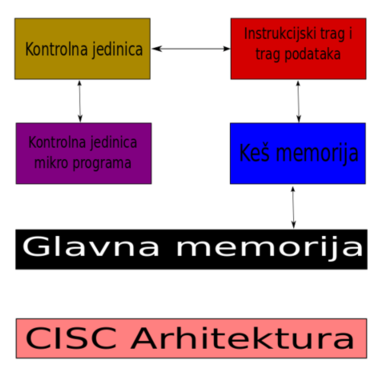
\includegraphics[scale=0.75]{cisc.png}
\end{center}
\caption{\textit{CISC} архитектура}
\label{fig:main}
\end{figure}

\begin{figure}[h!]
\begin{center}
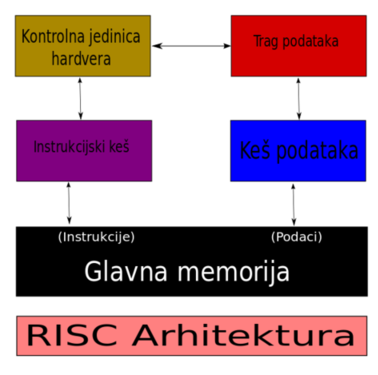
\includegraphics[scale=0.75]{risc.png}
\end{center}
\caption{\textit{RISC} архитектура}
\label{fig:main}
\end{figure}

\indent \textit{CISC} архитекуру процесора карактерише богат скуп инструкција. Овај приступ имеплементације хардвера покушава да смањи број инструкција по програму, жртвовањем броја циклуса по инструкцији. Рачунари засновани на \textit{CISC} архитектури су дизајнирани да смањују трошкове меморије. Великим програмима је потребно много меморије, чиме се повећава трошак меморије и велика меморија постаје скупља. Да би се решио овај проблем, број инструкција по програму може бити смањен уградњом више операција у једну инструкцију, правећи тако комплексније инструкције~\cite{rcRef}.

\indent \textit{RISC} архитектура користи високо оптимизован скуп инструкција. Код \textit{RISC} архитектуре мотив је обрнут у односу на \textit{CISC} архитекуру, смањује се број циклуса по инструкцији по цени броја инструкција по програму. Проточна обрада (енг. \textit{pipeline}) је једна од јединствених одлика архитектуре \textit{RISC}, која је постигнута преклапањем извршавања неколико инструкција. Због проточне обраде \textit{RISC} архитектура има велику предност у перформансама у односу на \textit{CISC} архитектуре~\cite{rcRef}.



\section{\textit{MIPS}}
\label{sec_mips}

\indent \textit{MIPS} је \textit{RISC} архитектура процесора, рођена у плодном периоду академских истраживања и развоја, осамдесетих година прошлог века. \textit{MIPS} пројекат је један од пионирских пројеката на Стандфорду, на ком је радио Џон Хенеси са својим студентима.

\indent Релативна једноставност је била комерцијална нужност за \textit{MIPS} процесоре, која се 1985. године развила из академског пројекта за израду и пласира на тржиште чипова. Као резултат, ова архитектура је имала (можда још увек има) највећи ранг произвођача у индустрији, прозводећи од \textit{ASIC} језгара (\textit{MIPS Technologies}) до веома јефтиних процесора (\textit{IDT, AMD/Alchemy}), укључујући и само 64-битне процесоре (\textit{PMC-Sierra, Toshiba, Broadcom}).

\indent Процесори засновани на \textit{MIPS} скупу инструкција се често користе код наменских уређаја и ручних рачунара (енг. \textit{handheld PC}). Мобилни уређаји, сет-топ боксови, паметни телевизори, за које се често користе \textit{MIPS} процесори, повлаче са собом велики број апликација са интензивним израчунавањем као што су: процесирање слике и видеа, интеракција између човека и компјутера, анализа података...

\section{Регистри у MIPS-у}
\label{registri}

\indent Регистри представљају малу, веома брзу меморију, која је део процесора. \textit{MIPS} процесори могу вршити операције само над садржајима регистара и специјалним константама које су део инструкције. \\
\indent У архитектури \textit{MIPS}, постоји 32 регистара опште намене. Само два регистара се понашају другачије од осталих регистара:

\begin{description}
  \item[\$0] - Увек враћа нулу, без обзира којa му се вредност додели
  \item [\$31] - Увек се користи за адресу повратка из функције на коју се скочи инструкцијом \textit{jal}
\end{description}
Сви ови регистри се могу користити за било коју инструкцију (може се чак користити и регистар \$0 као дестинација, мада ће резултат да нестане). 

Регистри опште намене су описани у наставку:
\begin{description}
  \item[at] - Резервисан за псеудоинструкције које асемблер генерише
  \item[v0, v1] - Користе се за враћање резултата при повратку из неке функције. Резултат може бити целобројног типа или број записан у фиксном зарезу.
  \item[а0 - а3] - Користе се за прослеђивање прва четири аргумената функције која се позива.
  \item[t0 - t9] - Користе се као привремени регистри. 
  \item[s0 - s7] - Садржај ових регистара мора остати непромењен након извршавања сваке функције, што се постиже привременим чувањем ових регистара на стеку уколико се њихова вредност мења у току функције и враћањем након завршетка функције. Ово су регистри које чува позвана функција (енг. \textit{calee saved registers}).
  \item[k0, k1] - Резервисано за систем прекида, који након коришћења не враћа садржај ових регистара на почетни. Систем прекида прво сачува садржаје регистара опште намене, који су важни за програм који се у том тренутку извршавао, и чији садржај планира да мења. У те сврхе се користе ови регистри.
  \item[gp] - Користи се у различите сврхе. У коду коjи не зависи од позициjе (енг. \textit{Position Independent Code} скраћено \textit{PIC}), регистар \textit{\$gp} показуjе на табелу показивача, познате као \textit{GOT} (скраћено од енг. Global Offset Table), преко које приступа деловима кода и подацима. \textit{PIC} је к\^{о}д који се може извршавати на било којој меморијској адреси, без модификација. PIC се најчешће користи за дељене библиотеке, при чему се заједнички к\^{о}д библиотеке може учитати у одговарајуће локације адресних простора различитих програма који је користе. \\
  У регуларном коду који зависи од позиције, регистар \textit{\$gp} се користи као показивач на средину у статичкој меморији. То значи да се подацима који се налазе 32 КВ лево или десно од адресе која се налази у овом регистру може приступити помоћу једне инструкције. Дакле, инструкције \textit{load} и \textit{store} које се користе за учитавање, односно складиштење података, се могу извршити у само једној инструкцији, а не у две као што је иначе случај. У пракси се на ове локације смештају глобални подаци који не заузимају много меморије. Оно што је битно је да овај регистар не користе сви системи за компилацију и сва окружења за извршавање.
  \item[sp] - Показивач на стек. Оно што је битно је да стек расте наниже. Потребне су специјалне инструкције да би се показивач на стек повећао и смањио, тако да \textit{MIPS} ажурира стек само при позиву и повратку из фукције, при чему је за то одговорна функција која је позвана. \textit{sp} се при уласку у функцију прилагођава на најнижу тачку на стеку којој ће се приступати у функцији. Тако је омогућено да компајлер може да приступи поменљивама на стеку помоћу константног помераја у односу на \textit{\$sp}.
  \item[fp] - Познат и као \textit{\$sp}, показивач на стек оквир. Користи се од стране функције, за праћење стања на стеку, за случај да из неког разлога компајлер или програмер не могу да израчунају померај у односу на \textit{\$sp}. То се може догодити уколико програм врши проширење стека, при чему се вредност проширења рачуна у току извршавања. Ако се дно стека не може израчунати у току превођења, не може се приступити променљивама помоћу \textit{\$sp}, па се на почетку функције \textit{\$fp} иницијализује на константну позицију која одговара стек оквиру функције. Ово је локално за функцију.
  \item[ra] - Ово је подразумевани регистар за смештање адресе повратка и то је подржано кроз одговарајуће инструкције скока. Ово се разликује од конвеције која се користи на архитеткури x86, где инструкција позива функције адресу повратка смешта на стек. При уласку у функцију регистар \textit{ra} обично садржи адресу повратка функције, тако да се функције углавном завршавају инструкцијом \textit{jr \$ra}, али у принципу, може се користити и неки други регистар. Због неких оптимизација које врши процесор, препоручује се коришћење регистара \textit{\$ra}. Функције које позивају друге функције морају сачувати садржај регистара \textit{\$ra}.
\end{description}


\section{Регистри за рад са бројевима у покретном зарезу у \textit{MIPS}-у}
\label{fp_registri}

Архитектура \textit{MIPS} користи два формата \textit{FP} (скр. \textit{Floating Point}) препоручена од стране IEEE 754:

\begin{itemize}
	\item \textit{Једнострука прецизност} (eнг. \textit{Single precision}) - Користи се 32 бита за чување у меморији. \textit{MIPS} компајлери користе једноструку прецизност за променљиве типа \textit{float}
	\item \textit{Двострука прецизност} (eнг. \textit{Double precision}) - Користи се 64 бита за чување у меморији. \textit{C} компајлери користе двоструку прецизност за C \textit{double} типове података.
\end{itemize}

\indent Начин на који се 64-битна реч смешта у меморију, односно две речи од којих се он састоји, зависи од начина на који процесор смешта податке у меморију ( нижи бит на нижој адреси или виши бит на нижој адреси). 

\indent Стандард IEEE 754 је веома захтеван и поставио је два велика проблема. Први проблем омогућавање детекције неуобичајних резултата, доводи проточну обраду тешком. Постоји опција да се имплементира IEEE механизам сигнализирања изузетака, али је проблем да се детектују случајеви када хардвер не може да произведе исправан резултат и потребна му је помоћ.

\indent Када се IEEE изузетак деси требало би обевестити и корисника, ово би требало бити синхроно; након заустављања стање \textit{FP} регистара је исто као и пре почетка извршавања инструкције која је довела до изузетка.

\indent У архитектури \textit{MIPS}, хардверска заустављања су имплементирана на начин који је описан. Ово заправо ограничава могућности проточне обраде \textit{FP} операција, јер се не може извршити следећа инструкције све док хардвер није сигуран да следећа \textit{FP} операција неће произвести заустављање. Зарад избегавања додавања времена за извршавање, \textit{FP} операције морају да одлуче да ли ће доћи до заустављања у првој фази. 

\indent \textit{MIPS} процесори имају 32 \textit{FP}, који су обично обележени \textit{\$f0 - \$f31}. Са изузетком неких јако старих процесора као што је \textit{MIPS I}, сваки 64-битни регистар може да садржи вредност двоструке прецизности.

\indent Први \textit{MIPS} процесор је имао 16 регистара. Заправо, постајало је 32 32-битних регистара, али од сваког пара парно/непарних регистара направљена је јединица за математичке операције (укључујући и математичке операције за двоструку прецизност). Непарни регистри се користе за операције учитавања, чувања и премештања између \textit{FP} регистара и регистара за целобројне вредности.

\indent \textit{MIPS I} је избачен из употребе, али касније верзије процесора имају такозвани "бит компатибилности" у регистру \textit{SR(FR)}. Уколико се у овај регистар постави вредност нула добијају се операције за процесор \textit{MIPS I}. Још увек је у употреби велики број софтвера који раде на овај начин. Да би програм могао да користи \textit{FP} регистре мора да постоји подршка компајлера, као и да цео систем на ком желимо да покренемо програм буде конзистентности са коришћењем \textit{FP} регистара.

\indent \textit{MIPS FP} регистри се такође користе за чување и манипулацију означених целобројних вредности (32 и 64 битних). Тачније, када у програму постоји конверзија из целобројне вредности у бројеве са покретним зарезом, све те операције конверзије користе само \textit{FP} регистре - целобројна вредност у  \textit{FP} регистру је конвертована у вредност у покрентом зарезу у  \textit{FP} регистру~\cite{SeeMIPSRun}.

\section{Конвенција \textit{FPXX}}
\label{sec_fpxx}

\indent \textit{MIPS О32 ABI} је 32-битни скуп инструкција и правила за архитектуру \textit{MIPS} процесора. Конвенција \textit{FPXX} је додатак \textit{MIPS О32 ABI} скупу правила и дефинише услове које треба да задовољи машински програм како би се коректно извршавао независно од режима у коме ради јединица за операције са бројевима у покретном зарезу. Програмски к\^{о}д који поштује ову конвенцију практично користи подскуп инструкција које су заједничке за оба режима и као такав није оптималан, али је погодан за комбиновање са кодом превединим за било који режим рада у покретном зарезу. Идеја је да дељене библиотеке и кориснички програми који треба да буду портабилни, буду преведени у складу са конвенцијом \textit{FPXX}.


\indent \textit{MIPS ABI} је мењан током времена како се мењала архитекура. Промене које су настале у архитектури захтевале су да се преиспита стање \textit{О32 ABI} и процени да ли постоји могућност да се направи \textit{ABI} који би био компатибилан са тадашњим и свим будућим унапређивањима архитекуре. Три главна разлога за проширивање \textit{О32 ABI}-ја су била увођење \textit{MSA ASE} (\textit{MSA} је проширење архитектуре \textit{MIPS} модулом \textit{SIMD}, нове инструкције омогућавају евификасно паралелно извршавање векторских операција~\cite{MSA}), жеља да се искористи \textit{FR=1} режим \textit{FPU}-а и \textit{MIPS32r6} архитектура која подржава само \textit{FR=1} режим~\cite{fpxxRef}.

\begin{description}
\item[FR=0 режим (FP32)] описује \textit{FPU} са 32 32-битне регистре. Ови регистри су нумерисани од \$f0 до \$f31. Парови парних и непарних регистара се користе за добијење 64-битних контејнера и нумерисани су \$f0 до \$f30. Операције двоструке прецизности не смеју да користе непарне регистре.
\item[FR=1 режим (FP64)] описује \textit{FPU} који има 32 64-битна регистра. Ови регистри су нумерисани од \$f0 до \$f31 и сваки од њих се може користити и за вредности једноструке и двоструке прецизности. Када се користе за операције са једноструком прецизношћу виших 32-бита постаје недефинисано.
\item[FRЕ=1 режим] је уведен са процесором \textit{MIPS32r5}. Овај режим се користи у конјункцији са \textit{FR=1} режимом, \textit{FPU} има 32 64-битна регистра али је понашање одређених инструкција као у \textit{FR=0} режиму. Операције са 64-битним или ширим форматима се извршавају на исти начин као да се извршавају у \textit{FR=1} режиму, али 32-битни формати имају понашање као у \textit{FR=0} режиму. Посебна карактеристика \textit{FRЕ} режима се врти око руковања регистара са прецизношћу од 32-бита и понашање посебно са непарним регистрима. Да би се \textit{FP32} режим извршавао коректно када се користе непарни регистри мора да се ажурира виши 32-битни део парног 64-битног регистра, такође ажурирање парних 64-битних регистара има за последицу ажурирање непарних 32-битних регистара. \textit{FRЕ} режим ово достиже тако што преусмерава читање и писање са непарних регистара на горњих 32-бита парних регистара.
\end{description}

\indent Прве верзије \textit{MIPS}-a су подржавале само 32-битни копроцесор, док код осталих верзија ко-процесор може бити и 32-битни и 64-битни. Приликом писања програма програмер, односно компајлери који се користе морају да буду свесни у ком режиму ће се извршавати програм и у складу са тим да бирају инструкције које ће се користити. Додате су нове опције приликом превођења програма за одабир једног од три режима, приказаних у табели \ref{tbl:opcije}.


\begin{table}
\centering
\caption{Опције за превођење програма}
\label{tbl:opcije}
\begin{tabular}{ |c|p{10cm}| }
Опције & Значење \\\midrule
-mfp32 & Генерише се к\^{о}д који претпоставља да ће радити само на FP=0 FPU процесору \\
-mfpxx & Генерише се к\^{о}д који може да се улинкује са к\^{о}д који је преведен са опцијом -mfp32 или -mfp64 и може да се покрене на FP=0 или FP=1 FPU процесору \\
-mfp64 & Генерише се к\^{о}д који претпоставља да ће радити само на FP=1 FPU процесору \\
\end{tabular}
\end{table}

\indent Паралелно са увођењем конвенције \textit{FPXX} уведена је и  \textit{.MIPS.abiflags} секција објектног фајла. Ова секција садржи структуру података која представља суштинске информације које омогућавају одређивање, између осталог и, режима у ком програм ради. У табели \ref{tbl:fpabi} у колони Опције су представљене опције са којима се преводи програм, док у колони \textit{FP\_ABI} су вредности које се том приликом уписују у одговарајуће поље \textit{.MIPS.abiflags} секције објектног фајла. Приликом одлучивања у ком режиму ће радити програм, језгро чита вредност \textit{FP\_ABI} из самог програма као и из интерпретера уколико се ради о динамички преведеном програму. На основу те две вредности се у језгру одлучује у ком режиму ће програм радити. На пример, ако је програм преведен са опцијама -mabi=32 -mfp32 (FP\_ABI = 1), а интерпретер са опцијама  -mabi=32 -mfpxx (FP\_ABI = 5) процес ће започети рад у режиму FR = 0. Ако је програм преведен са опцијама -mabi=32 -mfpxx -modd-spreg (FP\_ABI = 6), а интерпретер са опцијама  -mabi=32 -mfpxx (FP\_ABI = 5) процес ће започети рад у режиму FR = 1.


\begin{table}
\centering
\caption{Опције за превођење програма и вредности променљиве \textit{FP\_ABI}}
\label{tbl:fpabi}
\begin{tabular}{ |c|c| }
Опције & \textit{FP\_ABI} \\\midrule
-mabi=32 -mfp32 & 1 \\
-mabi=64 -mfp64 & 1 \\
-msingle-float  & 2 \\
-msoft-float    & 3 \\
-mabi=32 -mfpxx & 5 \\
-mabi=32 -mfp64 -modd-spreg & 6 \\
-mabi=32 -mfp64 -mno-odd-spreg & 7 \\
\end{tabular}
\end{table}

\indent Инструкција \textit{mtc1} копира вредност из \textit{GP} регистра у \textit{FP} регистар, тачније нижих 32-бита из \textit{GP} регистра  преписује у нижих 32-бита \textit{FP} регистра. Инструкција \textit{mfc1} копира вредност из \textit{FP} у \textit{GP} регистар~\cite{MIPSInstrSet}. Инструкције \textit{mtc1} и \textit{mfc1} се не смеју користити за приступање вишег дела регистара двоструке прецизности. Уколико је потребно ове инструкције се могу користити за приступ нижем делу регистра двоструке прецизности. Сваки пренос 64-битних података између \textit{GP} и \textit{FP} регистара двоструке прецизности мора се радити кроз меморију. Архитектуре коjе подржаваjу инструкциjе \textit{MTHC1/MFHC1} могу оптималније приступити вишем делу регистара двоструке прецизности~\cite{fpxxRef}. Инструкција \textit{MTHC1} копира садржај из \textit{GP} регистра у горњих 32-бита \textit{FP} регистра, док инструкција \textit{MFHC1} копира горњих 32-бита из \textit{FP} регистра у \textit{GP} регистар~\cite{MIPSInstrSet}.

\indent Системски позив \textit{prctl()} се позива са првим аргументом који говори шта треба да се ради, док остали зависе умногоме од првог аргумента. Од верзије језгра 4.1 системском позиву \textit{prctl()} додате су две нове опције којима се може одредити и променити тренутни режим \textit{FPU} регистара.  Опцијом \textit{PR\_GET\_FP\-\_MODE} \textit{prctl()} системски позив нам враћа режим, док са опцијом \textit{PR\_SET\_FP\-\_MODE} можемо да мењамо тренутни режим рада. \textit{Рrctl()} системски позив може да контролише тренутни регистарски режим - режим се може погледати и нови режим може бити постављен. \textit{Рrctl()} системски позив може да промени режим свих нити које су у том тренутку активне~\cite{prctlRef}.


% ------------------------------------------------------------------------------
\chapter{Алат \textit{Valgrind}}
\label{chp:valgrind}

\indent \textit{Valgrind} је платформа за прављење алата за динамичку бинарну анализу кода. Динамичка анализа обухвата анализу корисничког програма у извршавању, док бинарна анализа обухвата анализу на нивоу машинског кода, снимљеног или као објектни к\^{о}д (неповезан) или као извршни к\^{о}д (повезан). Постоје \textit{Valgrind} алати који могу аутоматски да детектују проблеме са меморијом, процесима као и да изврше оптимизацију самог кода. \textit{Valgrind} се може користити и као алат за прављење нових алата. \textit{Valgrind} дистрибуција тренутно броји следеће алате: детектор меморијских грешака (\textit{Memcheck}), детектор грешака нити (\textit{Helgrind}), оптимизатор брзе меморије и скокова (\textit{Cachgrind}), генератор графа скривене меморије и предикције скока (\textit{Callgrind}) и оптимизатор коришћења динамичке меморије (\textit{Massif}). \textit{Valgrind} ради на следећим архитектурама:
\begin{description}
	\item[Linux] - \textit{x86}, \textit{AMD64}, \textit{ARM}, \textit{ARM64}, \textit{PPC32}, \textit{PPC64}, \textit{S390X}, \textit{MIPS32}, \textit{MIPS64}
	\item[Solaris] - \textit{x86}, \textit{AMD64}
	\item[Android] - \textit{ARM}, \textit{ARM64},\textit{x86} (4.0 и новије), \textit{MIPS32}
	\item[Darwin] - \textit{x86}, \textit{AMD64}(Mac OS X 10.12)
\end{description}

\indent У наредним поглављима биће детаљно описана структура \textit{Valgrind}-а и његових алата, као и начин употребе са примерима проблема са којима се програмери свакодневно сусрећу. У поглављу \ref{section_memcheck} биће описан алат \textit{Memcheck}, у поглављу \ref{section_cachgrind} ће бити више речи о алату \textit{Cachgrind}, у поглављу \ref{section_helgrind} су описани алати \textit{Helgrind} и \textit{DRD}, у поглављу \ref{section_callgrind} описан је алат \textit{Callgrind}, у поглављу \ref{section_massif} биће речи о алату \textit{Massif}.

\section{O Valgrind-u}

\indent Алат за динамичку анализу кода се креира као додатак, писан у \textit{C} програмском језику, на језгро \textit{Valgrind}-а. 


\begin{center}
\textit{Језгро Valgrind-a + алат који се додаје = Алат Valgrind-a} 
\end{center}


\indent Језгро \textit{Valgrind}-а омогућава извршавање клијентског програма, као и снимање извештаја који су настали приликом анализе самог програма. 

\indent Алати \textit{Valgrind}-а користе методу бојења вредности. Они заправо сваки регистар и меморијску вредност "боје" (замењују) са вредношћу која говори нешто додатно о оригиналној вредности. 

\indent Сви \textit{Valgrind} алати раде на истој основи, иако информације које се емитују варирају. Информације које се емитују могу се искористити за отклањање грешака, оптимизацију кода или било коју другу сврху за коју је алат дизајниран.

\indent Сваки \textit{Valgrind}-ов алат је статички повезана извршна датотека која садржи к\^{о}д алата и к\^{о}д језгра. Извршна датотека \textit{valgrind} представља програм омотач који на основу -\--tool опције бира алат који треба покренути. Извршна датотека алата статички је линкована тако да се учитава почев од неке адресе која је обично доста изнад адресног простора који користе класичан кориснички програм (на \textbf{\textit{x86/Linux}} и \textbf{\textit{MIPS/Linux}} користи се адреса 0x38000000). \textit{Valgrind}-ово језгро прво иницијализује подсистем као што су менаџер адресног простора, и његов унутрашњи алокатoр меморије и затим учитава клијентову извршну датотеку. Потом се иницијализују \textit{Valgrind}-ови подсистеми као што су транслациона табела, апарат за обраду сигнала, распоређивач нити и учитавају се информације за дебаговање клијента, уколико постоје. Од тог тренутка \textit{Valgrind} има потпуну контролу и почиње са превођењем и извршавањем клијентског програма. Може се рећи да \textit{Valgrind} врши JIT (\textit{Just In Time}) превођење машинског кода програма у машински к\^{о}д програма допуњен инструментацијом. Ниједан део кода клијента се не извршава у свом изворном облику. Алат се умеће у оригинални к\^{о}д на почетку, затим се нови к\^{о}д преводи, сваки основни блок појединачно, који се касније извршава. Процес превођења се састоји из рашчлањивања оригиналног машинског кода у одговарајућу међурепрезентацију (енгл. \textit{intermediate representation}, скраћено IR) који се касније инструментализује са алатом и поново преводи у нови машински код. 

\indent Резултат свега овога се назива транслација, која се чува у меморији и која се извршава по потреби. Језгро троши највише времана на сам процес прављења, проналажења и извршавања транслације. Оригинални к\^{о}д се никада не извршава. Једини проблем који се овде може догодити је ако се врши транслација кода који се мења током извршавања програма.

\indent Постоје многе компликације које настају приликом смештања два програма у један процeс (клијентски програм и програм алата). Многи ресурси се деле између ова два програма, као што су регистри или меморија. Такође, алат \textit{Valgrind}-а не сме да се одрекне тоталне контроле над извршавањем клијентског програма приликом извршавања системских позива, сигнала и нити.

\subsection{Основни блок}

\indent \textit{Valgrind} дели оригинални к\^{о}д у секвенце које се називају основни блокови. Основни блок је праволинијска секвенца машинског кода, на чији се почетак скаче, а која се завршава са скоком, позивом функције или повратком у функцију позиваоца. Сваки к\^{о}д програма који се анализира поново се преводи на захтев, појединачно по основним блоковима, непосредно пре самог извршавања самог блока. Ако узмемо да су основни блокови клијентског кода \textit{BB1, BB2, ...} онда преведене основне блокове обележавамо са \textit{t(BB1), t(BB2), ...} Величина основног блока је ограничена на максимално шесдесет машинских инструкција. На процесорима \textit{MIPS}, инструкције скока и гранања имају такозвано "одложено извршавање". То значи да се приликом извршавања тих инструкција извршава и инструкција која се налази непосредно иза инструкције гранања или скока. У случају да је последња шесдесета инструкција основног блока инструкција гранања, \textit{Valgrind} учитава и инструкцију која се налази непосредно иза ње, односно шесдесет и прву инструкцију. Тиме се омогућава конзистентно извршавање програма који се анализира, као и у случају да се програм извршава без посредства \textit{Valgrind}-а. Уколико након извршених шесдесет инструкција \textit{Valgrind} није наишао на инструкцију гранања, секвенца инструкција се дели на два или више основних блокова, који се извршавају један за другим.



\subsection{Системски позиви}

\indent Програми комуницирају са оперативним системом помоћу системских позива (eнг. \textit{system calls}), тј. преко операција (функција) које дефинише оперативни систем.

\indent Системски позиви се реализују помоћу система прекида: кориснички програм поставља параметре системског позива на одређене меморијске локације или регистре процесора, иницира прекид, оперативни систем преузима контролу, узима параметре, извршава тражене радње, резултат ставља на одређене меморијске локације или у регистре и враћа контролу корисничком програму.

\indent Апликација која жели да користи неке од ресурса, као што су меморија, процесор или улазно/излазни уређаји, комуницира са језгром опративног система користећи системске позиве. Језгро оперативног система дели виртуелну меморију на корисничку меморију и системску меморију. Системска меморија је одређена за само језгро оперативног система, његова проширања, као и за управљачке програме. Кориснички простор је део меморије где се налазе све корисничке апликације приликом њиховог извршавања. Корисничке апликације могу да приступе улазно/излазним уређајима, виртуалној меморији, датотекама и другим ресурсима језгра оператвиног система користећи само системске позиве. Системски позиви обезбеђују спрегу између програма који се извршава и оператвиног система. Генерално, реализују се на асемблерском језику, али новији виши програсмки језици, попут језика \textit{C} и \textit{C++}, такође омогућавају реализацију системског позива. Програм који се извршава може проследити параметре опративном систему на више начина, прослеђивање параметара у регистрима процесора, постављањем параметара у меморијској табели. Aдреса табеле се прослеђује у регистру процесора, постављањем параметара на врх стека (енг. \textit{push}), које оператвни систем "скида" (енг. \textit{pop}).

\indent Системски позиви се извршавају без посредства \textit{Valgrind}-а, зато што језгро \textit{Valgrind}-а не може да прати њихово извршавање у самом језгру оперативног система.


\subsection{Транслација}

\indent У наставку су описани кораци које \textit{Valgrind} извршава приликом анализе програма. Постоји осам фаза транслације. Све фазе осим инструментације коју обавља алат \textit{Valgrind}-а, обавља језгро \textit{Valgrind}-а.

\begin{description}
	\item[Дисасемблирање] - Процес превођења машинског кода у еквивалентни асемблерски код. \textit{Valgrind} врши превођење машинског кода у интерни скуп инструкција која се називају међукод инструкције. Међукод представља редуковани скуп инструкција (скр. енг. \textit{RISC}). Ова фаза је зависна од архитектуре на којој се извршава.
	\item[Оптимизација 1] - Прва фаза оптимизације линеаризује \textit{IR} репрезентацију. Примењују се неке стандардне оптимизације програмских преводилаца као што су уклањање редудантног кода, елиминација подизраза, једноставно одмотавање петљи и сл.
	\item[Инструментација] - Блок кода у \textit{IR} репрезентацији се прослеђује алату, који може произвољно да га трансформише. Приликом инструментације алат у задати блок додаје додатне \textit{IR} операције, којима проверава исправност рада програма.
	\item[Оптимизација 2] - Друга фаза оптимизације је једноставнија од прве, укључује множење констати и уклањање мртвог кода.
	\item[Градња стабла] - Линеаризована \textit{IR} репрезентација се конвертује натраг у стабло ради лакшег избора инструкција.
	\item[Одабир инструкција] - Стабло \textit{IR} репрезентације се конвертује у листу инструкција које користе виртуалне регистре. Ова фаза се такође разликује у зависности од архитеткуре на којој се извршава.
	\item[Алокација регистара] - Виртуални регистри се замењују стварним. По потреби се уводе пребацивања у меморију. Не зависи од платформе, користи позив функција које налазе из који се регистара врши читање и у које се врши упис.
	\item[Асемблирање] - Изабране инструкције се енкодују на одговарајући начин и смештају у блок меморије. Ова фаза се такође разликује у зависности  од архитектуре на који се изршава~\cite{SeeMIPSRun}.
\end{description}

\section{Memcheck}
\label{section_memcheck}

\indent Меморијске грешке често се најтеже детектују, а самим тим и најтеже отклањају. Разлог томе је што се такви проблеми испољавају недетерминистички и није их лако репродуковати. \textit{Memcheck} је алат који детектује меморијске грешке корисничког програма. Како не врши анализу изворног кода већ машинског, \textit{Memcheck} има могућност анализе програма писаног у било ком језику.

\indent За програме писане у језицима C и C++ детектује уобичајне проблеме као што је приступање недопуштеној меморији, на пример преписивање блокова на хипу, преписивање врха стека и приступање меморији која је већ ослобођена. Алат детектује и коришћење неицијализованих вредности, вредности које нису иницијализоване или које су изведене од других неицијализованих вредности. Неисправно ослобађање хип меморије, као што је дупло ослобађање хип блокова или неупареног коришћења фукнција \textit{malloc/new/new[]} и \textit{free/delete/delete[]} је још један од проблема који алат \textit{Memcheck} детектује. Као и преклапање параметара прослеђених функцијама (нпр. преклапање \textbf{\textit{src}} и \textbf{\textit{dst}} показивача к\^{о}д фукнције \textbf{\textit{memcpy}}) и цурење меморије.

\indent Пуштање преведеног програма кроз \textit{Valgrind}, врши се извршавањем следеће линије у терминалу:

\begin{center}
 valgrind -\--tool=memcheck ./main
\end{center}

\indent -\--tool = опција одређује који алат ће \textit{Valgrind} пакет користити. Програм који ради под контролом \textit{Memcheck}-a je обично двадесет до сто пута спорији него када се извршава самостално, због транслације кода. Излазни програм је повећан за излаз који додаје сам алат \textit{Memcheck}, који се исписује на стандардном излазу за грешке~\cite{memcheckRef}.



\subsection{Коришћење неиницијализованих вредности}

\begin{figure}[h!]
\begin{center}
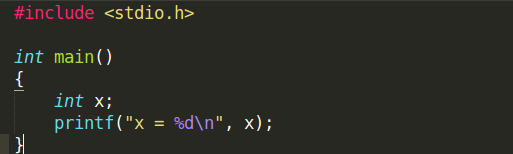
\includegraphics[scale=0.75]{slika1.png}
\end{center}
\caption{Пример програма који користи неиницијализовану променљиву}
\label{fig:main}
\end{figure}

\indent На слици \ref{fig:main} је дат пример програма у коме користимо неиницијализовану променљиву. Грешка у коришћењу неиницијализоване вредности се генерише када програм користи променљиве чије вредности нису иницијализоване.

\begin{figure}[h!]
\begin{center}
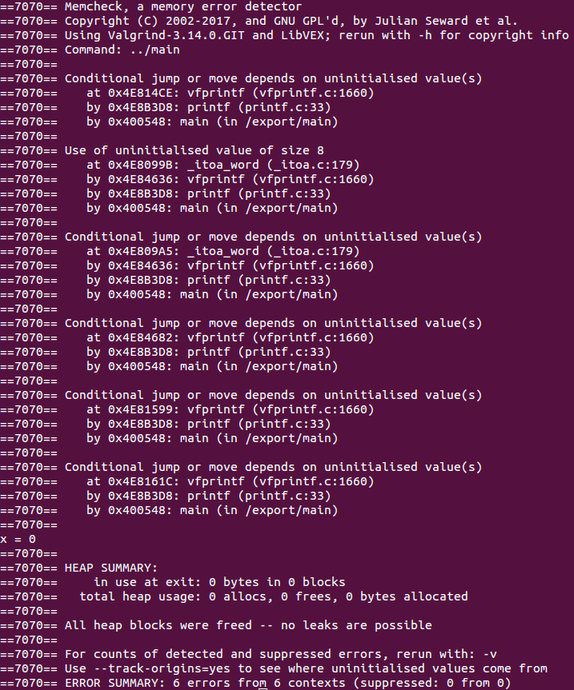
\includegraphics[scale=0.75]{slika2.png}
\end{center}
\caption{Детекција неиницијализованих вредности}
\label{fig:memcheck}
\end{figure}

\indent Слика \ref{fig:memcheck} приказује излаз \textit{Valgrind}-а који детектује коришћење неицијализованих вредности у програму. Први део, односно прве три линије се штампају приликом покретања било ког алата који је у склопу \textit{Valgrind}-а, у овом случају алата \textit{Memcheck}. Следећи део нам показује поруке о грешкама које је \textit{Memcheck} пронашао у програму. Последња линија приказује суму свих грешака које је алат пронашао и штампа се по завршетку рада. \\
\indent На овој слици је приказан излаз из \textit{Valgrind}-а када се открије  коришћење неицијализованих вредности. У програму неиницијализована променљива може више пута да се копира, \textit{Memcheck} прати све то, бележи податке о томе, али не пријављује грешку. У случају да се неиницијализоване вредности користе на начин да од те вредности зависи даљи ток програма или ако је потребно приказити вредности неиницијализоване променљиве, \textit{Memcheck} пријављује грешку. Да би могли да видимо главни извор коришћења неицијализованих вредности у програму, додаје се опција \textit{-\--trace-origins=yes}~\cite{memcheckRef}.

\subsection{Коришћење неиницијализоване или неадресиране вредности у системском позиву}

\indent \textit{Memcheck} прати све параметре системског позива.  Проверава сваки параметар појединачно, без обзира да ли је иницијализован или не. Проверава да ли системски позив треба да чита из меморије која је дефинисана у програму. \textit{Memcheck} проверава да ли је цела меморија адресирана и иницијализована. Ако системски позив треба да пише у меморију, \textit{Memcheck} проверава да ли је та меморија адресирана. После системског позива \textit{Memcheck} прецизно ажурира информације о промени у меморији које су постављене у системском позиву.

\begin{figure}[h!]
\begin{center}
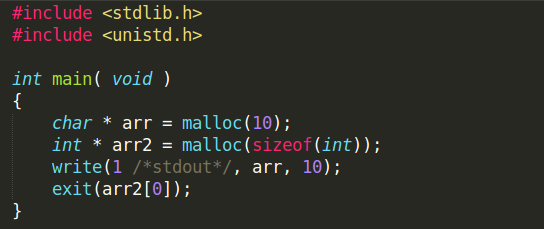
\includegraphics[scale=0.75]{slika3.png}
\end{center}
\caption{Пример позива системског позива са неисправним парамтрима}
\label{fig:main1}
\end{figure}



\begin{figure}[h!]
\begin{center}
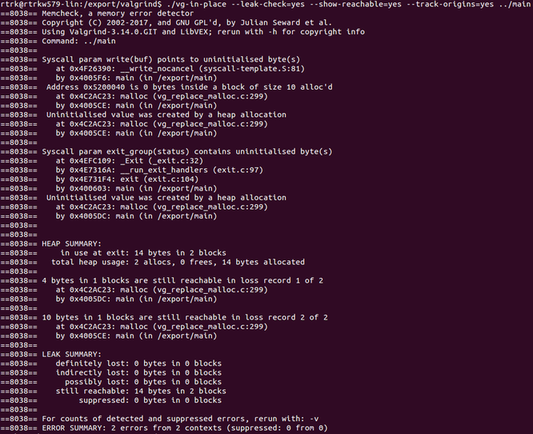
\includegraphics[scale=0.75]{slika4.png}
\end{center}
\caption{Пример излаза за програм који у себи садржи позив системског позива са неисправним парамтерима}
\label{fig:memcheck1}
\end{figure}

\indent На слици \ref{fig:main1} дат је пример позива системског позива са неисправним параметрима. На слици \ref{fig:memcheck1} је извештај који добијамо након анализе програма са слике \ref{fig:main1}. Можемо да видимо да је \textit{Memcheck} приказао информације о коришћењу неиницијализованих вредности у системским позивима. Прва грешка приказује да параметар системског позива \textit{write()} показује на неиницијализовану вредност. Друга грешка приказује да је податак који се прослеђује системском позиву \textit{exit()} недефинисан. Такође, приказане су и линије у самом програму где се ове вредности користе~\cite{memcheckRef}.

\subsection{Недопуштено ослобађање меморије}

\begin{figure}[h!]
\begin{center}
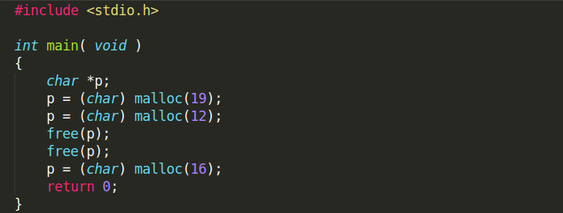
\includegraphics[scale=0.75]{slika5.png}
\end{center}
\caption{Пример нелаганог ослобађања меморије}
\label{fig:main2}
\end{figure}

\begin{figure}[h!]
\begin{center}
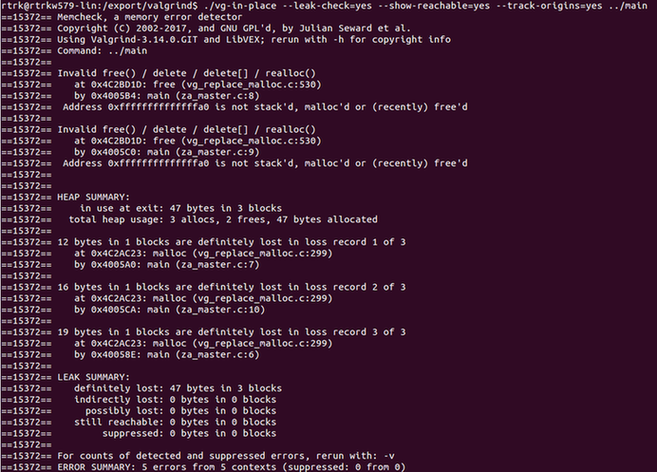
\includegraphics[scale=0.75]{slika6.png}
\end{center}
\caption{Пример излаза за програм у ком се нелагално ослобађа меморија}
\label{fig:memcheck2}
\end{figure}

\indent На слици \ref{fig:main2} дат је пример програма у коме се нелегално ослобађа меморија. \textit{Memcheck} прати свако алоцирање меморије које програм направи употребом функција \textit{malloc/new}, тако да он увек поседује информацију да ли су аргументи који се прослеђују функцијама \textit{free/delete} легитимни или не. У нашем примеру, програм ослобађа исту меморијску зону два пута. Извештај о недопуштеном ослобађању меморије приказан је на слици \ref{fig:memcheck2}.

\indent \textit{Memcheck} је пријавио да је програм покушао два пута да ослободи неку меморијску зону.  Такође, \textit{Memcheck} ће нам пријавити и ако програм покуша да ослободи меморијску зону преко показивача који не показује на почетак динамичке меморије~\cite{memcheckRef}.

\subsection{Детекција цурења меморије}

\indent \textit{Memcheck} бележи податке о свим динамичким блоковима који су алоцирани током извршавања програма позивом функција \textit{malloc(), new()} и др. Када програм прекине са радом, \textit{Memcheck} тачно зна колико меморијских блокова није ослобођено.

\indent Ако је опција \textit{-\--leak-check} адекватно подешена, за сваки неослобођени блок \textit{Memcheck} одређује да ли је могуће приступити том блоку преко показивача.

\indent Постоје два начина да приступимо садржају неког меморијског блока преко показивача. Први начин је преко показивача који показује на почетак меморијског блока. Други начин је преко показивача који показује на садржај унутар меморијског блока.

\indent Постоји неколико начина да сазнамо да ли постоји показивач који показује на унутрашњост неког меморијског блока. Први начин је да је постојао показивач који је показивао на почетак блока, али је намерно (или ненамерно) померен да показује на унутрашњост блока. Други начин, ако постоји нежељена вредност у меморији, која је у потпуности неповезана и случајна. И трећи начин, ако постоји показивач на низ C++ објеката (који поседују деструкторе) који су алоцирани са \textit{new[]}. У трећем случају, неки компајлери чувају "магични показивач" који садржи дужину низа од почетка блока.

\begin{figure}[h!]
\begin{center}
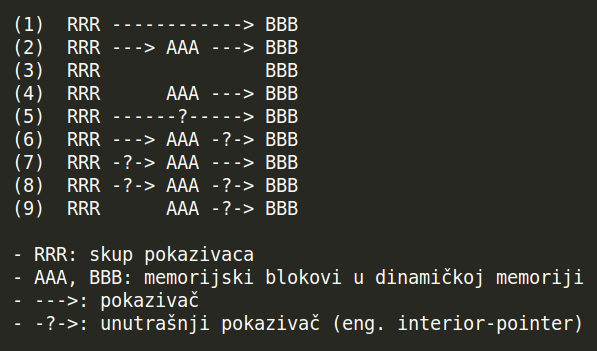
\includegraphics[scale=0.75]{slika7.png}
\end{center}
\caption{Пример показивача на меморијски блок}
\label{fig:memblok}
\end{figure}

\indent На слици \ref{fig:memblok} је приказано девет могућих случајева када показивачи показују на неке меморијске блокове. \textit{Memcheck} обједињује неке од ових случајева, тако да добијамо наредне четири категорије.

\begin{description}
  \item[Још увек доступан (енг. \textit{Still reachable}) ] - Ово покрива примере 1 и 2 на слици \ref{fig:memblok}. Показивач који показује на почетак блока или више показивача који показују на почетак блока су пронађени. Зато што постоје показивачи који показују на меморијску локацију која није ослобођена, програмер може да ослободи меморијску локацију непосредно пре завршетка извршавања програма.
  \item [Дефининитивно изгубљен (енг. \textit{Definitely lost})] - Ово се односи на случај 3 на слици \ref{fig:memblok}. Ово значи да је немогуће пронаћи показивач који показује на меморијски блок. Блок је проглашен изгубљеним, заузета меморија не може да се ослободи пре завршетка програма, јер не постоји показивач на њу.
  \item [Индиректно изгубљен (енг. \textit{Indirectly lost})] - Ово покрива случајеве 4 и 9 на слици \ref{fig:memblok}. Меморијски блок је изгубљен, не зато што не постоји показивач који показује на њега, него зато што су сви блокови који указују на њега изгубљени. На пример, ако имамо бинарно стабло и корен је изгубљен, сва деца чворови су индиректно изгубљени. С обзиром на то да ће проблем нестати ако се поправи показивач на дефинитивно изгубљен блок који је узроковао индиректно губљење блока, \textit{Memcheck} неће пријавити ову грешку уколико није укључена опција \textit{-\--show-reachable=yes}.
  \item [Могуће изгубљен (енг. \textit{Possibly lost})] - Ово су случајеви од 5 до 8 на слици \ref{fig:memblok}. Пронађен је један или више више показивача на меморијски блок,  али најмање један од њих показује на унутрашњост меморијског блока. То може бити само случајна вредност у меморији која показује на унутрашњост блока, али ово не треба сматрати у реду док се не разреши случај показивача који показује на унутрашњост блока.
\end{description}

\indent Ако постоји забрана приказивања грешке за одређени меморијски блок, без обзира којој од горе поменутих категорија припада, она неће бити приказана.

\begin{figure}[h!]
\begin{center}
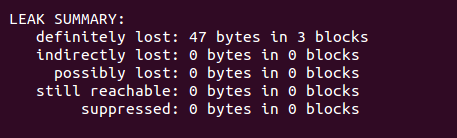
\includegraphics[scale=0.75]{slika8.png}
\end{center}
\caption{Резиме цурења меморије}
\label{fig:memcurenje}
\end{figure}

\begin{figure}[h!]
\begin{center}
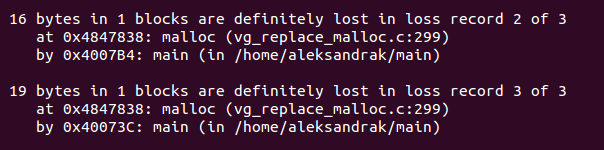
\includegraphics[scale=0.75]{slika9.png}
\end{center}
\caption{Извештај о цурењу меморије}
\label{fig:memizv}
\end{figure}


\indent На слици \ref{fig:memcurenje} је дат резиме цурења меморије који исписује \textit{Memcheck}. Ако је укључена опција \textit{-\--leak-check=yes}, \textit{Memcheck} ће приказати детаљан извештај о сваком дефинитивно или могуће изгубљеном блоку,  као и о томе где је он алоциран. \textit{Memcheck} нам не може рећи када, како или зашто је неки меморијски блок изгубљен. Генерано, програм не треба да има ниједну дефинитвно или могуће изгубљен блок на излазу.

\indent На слици \ref{fig:memizv} је приказан извештај који нам даје \textit{Memcheck} о дефинитивном губитку два блока величине 16 и 19 бајта, као и линију у програму где су они алоцирани.

\indent Због постојања више типова цурења меморије поставља се питање које цурење меморије на излазу из програма треба да посматрамо као "грешку", а коју не. \textit{Memcheck} користи следећи критеријум:

\begin{itemize}
  \item \textit{Memcheck} сматра да је цурење меморије "грешка" само ако је укључена опција \textit{-\--leak-check=full}. Другим речима, ако подаци о цурењу меморије нису приказани, сматра се да то цурење није "грешка".
  \item Дефинитивно и могуће изгубљени блокови се сматрају за праву "грешку", док индиректно изгубљени и још увек доспуни блокови се не сматрају као грешка~\cite{memcheckRef}.
\end{itemize}


\section{Cachgrind}
\label{section_cachgrind}

\indent \textit{Cachgrind} је алат који симулира и прати приступ брзој меморји машине на којој се програм, који се анализира, извршава. Он симулира меморију машине, која има први ниво брзе меморије подељене у две одвојене независне секције: \textit{I1} - секција брзе меморије у коју се смештају инструкције и \textit{D1} - секција брзе меморије у коју се смештају подаци. Други ниво брзе меморије коју \textit{Cachgrind} симулира је обједињен - \textit{L2}. Овај начин конфигурације одговара многим модерним машинама.

\indent Постоје машине које имају и три или четири нивоа брзе меморије. У том случају, \textit{Cachgrind} симулира приступ првом и последњем нивоу. Генерално гледано, \textit{Cachgrind} симулира  \textit{I1}, \textit{D1} и \textit{LL} (последњи ниво брзе меморије).

\indent \textit{Cachgrind} прикупља следеће статистичке податке о програму који анализира (скраћенице које се користе даље у тексту су дате у заградама):

\begin{itemize}
	\item  Подаци о читањима инструкција из брзе меморије укључују следеће статистике
\begin{description}
	\item[Ir] - укупан број извршених инструкција
	\item[I1mr] - број промашаја читања инструкција из брзе меморије нивоа \textit{I1}
	\item[ILmr] - број промашаја читања инструкција из брзе меморије нивоа \textit{LL}
\end{description}
	\item Подаци о читањима брзе меморије укључују следеће статистике
\begin{description}
	\item[Dr] - укупан број читања меморије
	\item[D1mr] - број промашаја читања нивоа брзе меморије \textit{D1}
	\item[DLmr] - број промашаја читања нивоа брзе меморије \textit{LL}
\end{description}
	\item Подаци о писањима у брзу меморију укључују следеће статистике
\begin{description}
	\item[Dw] - укупан број писања у меморији
	\item[D1mw] - број промашаја писања у ниво брзе меморије \textit{D1}
	\item[DLmw] - број промашаја писања у ниво брзе меморије \textit{LL}
\end{description}
	\item Број условно извршених грана (\textbf{Bc}) и број промашаја условно извршених грана (\textbf{Bcm}).
	\item Број индиректно извршених грана (\textbf{Bi}) и број промашаја индиректно извршених грана (\textbf{Bim}).
\end{itemize}
    
   

\indent Приметимо да је број приступа \textit{D1} делу брзе меморије једнак збиру \textit{D1mr} и \textit{D1mw}, док је укупан број приступа нивоу \textit{LL} једнак збиру  \textit{ILmr}, \textit{DLmr} и \textit{DLmw} броју приступа. Ова статистика се прикупља на нивоу целог програма, као и појединачно на нивоу функција. Може се такође, добити и број приступа скривеној меморији за сваку линију кода у оригиналном програму. На модерним машинама \textit{L1} промашај кошта око 10 процесорских циклуса, \textit{LL} промашај кошта око 200 процесорских циклуса, а промашаји условно и инидиректно извршене гране од 10 до 30 процесорских циклуса~\cite{cachegrindRef}.

\subsection{Коришћење \textit{Cachgrind}-a}

\indent На почетку коришћења алата \textit{Cachgrind}, програм који желимо да анализирамо покрећемо самим \textit{Cachgrind}-ом. На тај начин прикупљамо информације које су нам потребне за касније профилисање кода. Затим покрећемо алат \textit{cg\_annotate} у оквиру пакета \textit{Valgrind} који нам приказује детаљан извештај о програму који анализирамо са \textit{Cachgrind}-ом. Опционо, можемо да користимо алат \textit{cg\_merge} да сумирамо у једну датотеку више излаза које смо добили вишеструким покретањем \textit{Cachgrind}-а над истим програмом. Ту датотетку касније користимо као улаз у \textit{cg\_annotate}. Такође, можемо да користимо алат \textit{cg\_diff} који прави разлику између више излаза из алата \textit{Cachgrind}, које касније користимо као улаз у алат \textit{cg\_annotate}

\indent Покретање самог алата \textit{Cachgrind} врши се извршавањем следеће линије у терминалу:

\begin{center}
 valgrind -\--tool=cachgrind ./main
\end{center}


\begin{figure}[h!]
\begin{center}
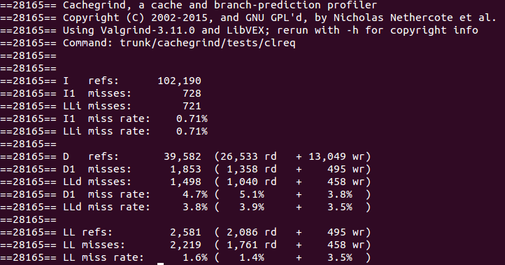
\includegraphics[scale=0.75]{slika10.png}
\end{center}
\caption{Извештај алата \textit{Cachgrind}}
\label{fig:cachgrind}
\end{figure}

\indent Извршавање програма кроз \textit{Cachgrind} траје веома споро. Након завршетка рада, добијају се статитстике као што је приказано на слици \ref{fig:cachgrind}~\cite{cachegrindRef}.

\subsection{\textit{Cachgrind} метаподаци}

\indent У наставку су описани метаподаци који се чувају у структурама.

\indent \textbf{Глобално стање брзе меморије}. Прва структура која се налази у склопу \textit{Cachgrind} метаподатака је глобано стање брзе меморије. Она представља три дела симулиране брзе меморије (\textit{L1}, \textit{D1},  \textit{LL}). Њене вредности се освежавају приликом извршене сваке инструкције програма чија се брза меморија симулира, тачније, приликом позива функције које симулирају приступ брзој меморији циљне платформе. Функцијама се прослеђују информације о приступу брзој меморији, као што су адресе и величина меморије којој се приступа.

\indent Симулација приступа брзој меморији има следеће карактеристике када се деси промашај уписа у брзу меморију, блок који је потребно уписати се смешта у \textit{D1} део брзе меморије. Инструкције које модификују вредности меморије третирају се као читање брзе меморије. Наиме, инструкције које мењају садржај брзе меморије најпре читају садржај брзе меморије, модификују вредност и снимају нову вредност. Самим тим, упис у брзу меморију не може да изазове промашај, јер је гарантован успешним читањем. Такође, циљ \textit{Cachgrind}-а није да прикаже колико пута се приступа брзој меморији, већ да прикаже број промашаја приступа брзој меморији. Линија у брзој меморији, којој одговара садржај у меморији са директним приступом, одређује се као $(M + N - 1)$, где је величина линије једнако 2 на M бајта, (величина брзе меморије / величина линијe) једнако је 2 на N бајта. \textit{L2} део брзе меморије реплицира све уносе у \textit{L1} део брзе меморије. Онај блок у брзој меморији који се најмање користи ће бити избачен из брзе меморије уколико је потребно убацити нови блок података у брзу меморију. Са референцама које показују на две линије у кеш меморији рукује се на следећи начин: уколико су пронађена оба блока у брзој меморији, рачунамо само један погодак, уколико један блок нађемо у брзој меморији, а други не, рачунамо један промашај (и нула погодатака) и уколико оба блока не пронађемо у брзој меморији, рачунамо један промашај (не два).

\indent Параметри симулиране брзе меморије (величина брзе меморије, величина линије и асоцијативност) одређују се на један од два начина. Први начин је употребом \textit{cpuid} наредбе. Други начин представља ручно уношење параметара симулиране брзе меморије, приликом покретања самог \textit{Cachgrind}.

\begin{figure}[h!]
\begin{center}
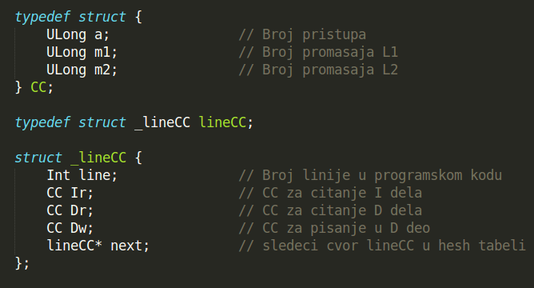
\includegraphics[scale=0.75]{slika11.png}
\end{center}
\caption{Структура централне табеле трошкова}
\label{fig:tabelaTroskova}
\end{figure}

\begin{figure}[h!]
\begin{center}
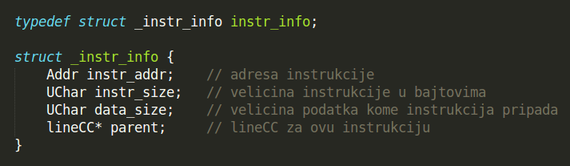
\includegraphics[scale=0.75]{slika12.png}
\end{center}
\caption{Структура табеле информација о инструкцијама}
\label{fig:infoInstr}
\end{figure}

\indent \textbf{Централна табела трошкова}. Друга структура која чини метаподатке алата \textit{Cachgrind} је централна табела трошкова. Свака линија у коду која се инструментализује, алоцира једну овакву табелу у коју смешта податке о приступу брзој меморији, броју погодака и промашаја приступа брзој меморији, који се дешавају приликом извршавања саме линије кода. На слици \ref{fig:tabelaTroskova} приказане су структуре које представљају централну табелу трошкова. \textit{ULong} је 64-битна целобројна вредност. Узимамо 64-битну вредност, јер број приступа може да буде већи него што може да се представи 32-битном целобројном вредношћу. У \textit{CC} структури \textit{m1} и \textit{m2} представљају број промашаја за \textit{L1} и \textit{LL} део брзе меморије. Структура \textit{lineCC} садржи три \textit{CC} елемента: за читање \textit{I} дела, за читање дела \textit{D} и за писање у део \textit{D} брзе меморије. Поље \textit{next} је потребно јер је централна табела трошкова представљена као променљива \textit{"heš"} табела. Поље \textit{line} представља број линије у коду која одговара тој табели трошкова. Сам број линије није довољан да би се пронашла линија у коду којој одговара централна табела трошкова (име фајла је потребно). У пракси, то значи централна табела трошкова има три новоа: трошкови су груписани по имену фајла, затим по имену функције и на крају по броју линије.


\indent \textbf{Табела информација о инструкцијама}. Трећа структура која чини метаподатке алата \textit{Cachgrind} је табела информација о инструкцијама. Она се користи за чување непроменљивих информација о самим инструкцијама током самог процеса инструментације. На овај начин се смањује величина додатог кода којим се анализира код. Повећава се брзина извршавања самог алата, јер се самњује број аргумената који се просеђују функцијама, које врше симулацију приступа брзој меморији.


\indent Свакој инструментализованој инструкцији додељује се по једно поље у табели информација о инструкцијама, које садржи структуру \textit{instr\_info}, приказаној на слици \ref{fig:infoInstr}. Поље \textit{instr\_addr} представља адресу инструкције,  \textit{instr\_size} представља величину инструкције изражену у бајтовима, \textit{data\_size} чува величину података коме инструкција приступа (0 уколико инструкција не приступа меморији) и \textit{parent} показује на поље у табели трошкова за исту линију кода одакле је инструкција изведена~\cite{cachegrindRef}.

\subsection{Инструментација}

\indent Први корак приликом инструментације кода односи се на пролаз кроз све основне блокове појединачно ради пребројавања инструкција које се налазе у њима. На основу овог броја се креира листа \textit{instr\_info} елемената, при чему сваки елемент листе одговара једној инструкцији у основном блоку.

\indent У другом пролазу, \textit{Cachgrind} врши категоризацију оригиналних инструкција. \textit{Cachgrind} дели инструкције у следеће категорије:

\begin{itemize}
  \item Инструкције које не приступају меморији, нпр. \textit{move \$t3, \$a0}
  \item Инструкције које читају садржај меморије, нпр. \textit{lw \$t3, 4(\$a0}
  \item Инструкције које уписују садржај регистара у меморију, нпр. \textit{sw \$t3, 4(\$a0)}
  \item Инструкције које модификују садржај меморијске локације
  \item Инструкције које читају садржај из једне меморијске локације и тај садржај уписују у другу меморијску локацију.
\end{itemize}

\indent Свака инструкција система базираног на \textit{MIPS} процесорима је растављена на више \textit{UCode} инструкција, тако да \textit{Cachgrind} одређује којој категорији оригинална инструкција припада на основу \textit{LOAD} и \textit{STORE} \textit{UCode} инструкција. \textit{Cachgrind} чита инфромације које помажу при отклаљању грешака. На основу ових информација он креира елементе \textit{lineCC} у централној табели трошкова. Затим иницијализује одређене \textit{instr\_info} елементе у  низ који је иницијализован за сваки основни блок појединачно (где је н-ти елемент \textit{instr\_info} одговара н-тој инструкцији у основном блоку). Када је иницијализовао све елементе \textit{lineCC} и \textit{instr\_info} алат \textit{Cachgrind} извршава процес инструментализације кода који се састоји из позива одговарајућих \textit{C} функција, које симулирају приступ брзој меморији циљне платформе. Која \textit{C} функција ће бити позвана зависи од категорије којој инструкција припада. Постоје само четири врсте \textit{C} функција које симулирају приступ брзој меморији, јер функције које припадају другој и четврој категорији позивају исту \textit{C} функцију за симулирање приступа брзој меморији. Број параметара који се прослеђује функцији програмског језика \textit{C} се, одређује на основу категорије којој та функција припада~\cite{cachegrindRef}.

\subsection{Приказ статистичких информација}

\indent Приликом завршетка анализе програма \textit{Cachgrind} похрањује прикупљену табелу трошкова у датотеку која се назива \textit{cachgrind.out.pid}; при чему \textit{pid} представља јединстевени идентификатор процеса који се извршио. Алат групише све трошкове по фајловима и функцијама којима ти трошкови припадају. Глобална статистика се рачуна накнадно, приликом приказа резултата. На овај начин се штеди јако пуно времана приликом анализе кода. Функције које симулирају приступ брзој меморији се позивају јако често, тако да би додавање још неколико инструкција које сабирају, знатно успорило и овако споро извршавање алата~\cite{cachegrindRef}.

\section{Helgrind и DRD}
\label{section_helgrind}

\indent \textit{Helgrind} је алат у склопу програмског пакета \textit{Valgrind} који открива грешке синхронизације приликом употребе модела нити \textit{POSIX}, док је \textit{DRD} алат за детекцију грешака у \textit{C} и \textit{C++} програмима који користе више нити. \textit{DRD} ради за сваки програм који користи нити \textit{POSIX} стандарда или који користе концепте који су надограђени на овај стандард.

\indent Главне апстракције модела нити \textit{POSIX} су: група нити која дели заједнички адресни простор, формирање нити, чекање за завршетак извршавања функције нити, излаз из функције нити, мутекс објекти, условне промељиве, читај-пиши закључавање и семафори.

\subsection{Лоша употреба интерфејса за програмирање нити \textit{POSIX}}

\indent Многе имплементације интерфејса су оптимизоване ради бржег времена извршавања. Такве имплементације се неће бунити на одређене грешке (ако мутекс откључа нека друга нит, а не она која га је закључала).

Грешке које \textit{Helgrind} и \textit{DRD} проналазе су:
\begin{itemize}
	\item Грешке у откључавању мутекса - када је мутекс неважећи, није закључан или је закључан од стране друге нити.
	\item Грешке у раду са закључаним мутексом - уништавање неважећег или закључаног мутекса, рекурзивно закључавање нерекурзивног мутекса, деалокација меморије која садржи закључан мутекс.
	\item Прослеђивање мутекса као аргумента функције која очекује као аргумент  \textit{reader-writer lock} и обрнуто.
	\item Грешке са \textit{pthread barrier} - неважећа или дупла иницијализација,  уништавање \textit{pthread barrier} који никада није иницијализован или кога нити чекају или чекање на објекат који није никада иницијализован.
	\item Грешке приликом коришћења функције \textit{pthread\_cond\_wait} - прослеђивање незакључаног, неважећег или мутекса кога је закључала друга нит.
	\item \textit{Pthread} функција врати к\^{о}д грешке који је потрено додатно обрадити, када се нит уништи, а да још држи закључану промељиву.
	\item Неконзистентне везе између условних промељивих и њихових одговарајућих мутекса. 
\end{itemize}

\indent Овакве грешке могу да доведу до недефинисаног понашања програма и до појаве грешака у програмима које је касније веома тешко открити. \textit{Helgrind} пресреће позиве ка функцијама библиотеке \textit{pthread}, и због тога је у могућности да открије велики број грешака. За све \textit{pthread} функције које \textit{Helgrind} пресреће, генерише се податак о грешци ако функција врати к\^{о}д грешке, иако \textit{Helgrind} није нашао грешке у коду.

\begin{figure}[h!]
\begin{center}
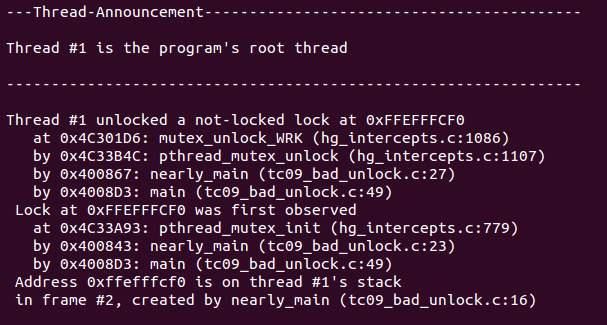
\includegraphics[scale=0.75]{slika13.png}
\end{center}
\caption{Пример приказа грешке у програму}
\label{fig:interfejs}
\end{figure}

\indent Провере које се односе на мутексе се такође примењују и на \textit{reader-writer lock}. Пријављена грешка приказује и примарно стање стека које показје где је детектована грешка. Такође, уколико је могуће исписује се и број линије у самом коду где се грешка налази. Уколико се грешка односи на мутекс, \textit{Helgrind} ће приказати и где је први пут детектовао проблематични мутекс \ref{fig:interfejs}~\cite{helgrindRef}.

\subsection{Потенцијално блокирање нити}

\indent \textit{Helgrind} прати редослед којим нити закључава промељиве. На овај начин \textit{Helgrind} детектује потенцијалне делове кода који могу довести до блокорања нити. На овај начин је могуће детектовати грешке које се нису јавиле током самог процеса тестирања програма, већ се јављају касније током коришћења истог.

\indent Илустрација оваквог проблема је дата у наставку.

\begin{itemize}
  \item Претпоставимо да је дељени објекат $O$ коме да би приступили морамо да закључамо две променљиве $M_1$ и $M_2$.
  \item  Замислимо затим да две нити $T_1$ и $T_2$ желе да приступе дељеној променљивој $O$. До блокорања нити долази када нит $T_1$ закључа $M_1$, а у истом тренутку $T_2$ закључа $M_2$. Након тога нит $T_1$ остане блокирана јер чека да се откључа $M_2$, а нит $T_2$ остане блокирана јер чека да се откључа $T_1$.
\end{itemize}


\indent \textit{Helgrind} креира граф који представља све променљиве које се могу закључати, а које је открио у прошлости. Када нит наиђе на нову променљиву коју закључава, граф се освежи и проверава се да ли граф садржи круг у коме се налазе закључане променљиве. Постојање круга у коме се налазе закључане променљиве је знак да је могуће да ће се нити некада у току извршавања блокирати. Ако постоје више од две закључане променљиве у кругу проблем је још озбиљнији~\cite{helgrindRef}.

\indent Алат \textit{DRD} не открива овај тип грешака.


\subsection{Трка за подацима}

\indent Трка за подацима може да се јави услед недостатка адекватног закључавања или синхронизације. Приступ подацима без адекватног закључавања или синхронизације се односи на проблем када две или више нити приступају дељеном податку без синхронизације. На овај начин је могуће да две или више нити у истом тренутку приступе дељеном објекту~\cite{helgrindRef}.

\indent На слици \ref{fig:main4} приказан је пример програма у ком се користи променљива без адекватне синхронизације.

\begin{figure}[h!]
\begin{center}
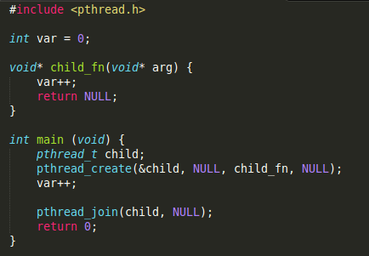
\includegraphics[scale=0.75]{slika14.png}
\end{center}
\caption{Пример приступа променљивој без адекватне синхронизације}
\label{fig:main4}
\end{figure}


\indent У овом примеру проблем настаје јер ништа не спречава нит родитељ и нит дете да у исто време приступе и промене вредност дељене променљиве \textit{var}. Приликом анализе оваквог програма алатом \textit{Helgrind} добија се извештај који је приказан на слици \ref{fig:helgrind}.

\indent У извештају који је приказан на слици \ref{fig:helgrind} можемо тачно да видимо које нити приступају променљивој без синхронизације, где се врши сам приступ променљивој, име и величину саме променљиве којој нити приступају ради промене њене вредности~\cite{helgrindRef}.

\begin{figure}[h!]
\begin{center}
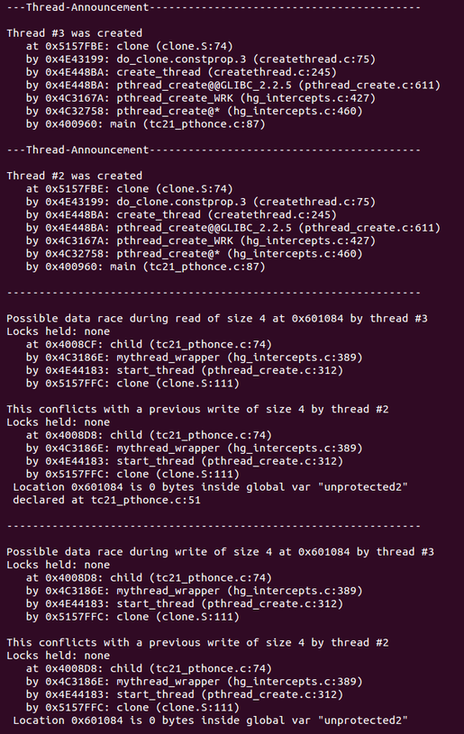
\includegraphics[scale=0.75]{slika17.png}
\end{center}
\caption{Извештај \textit{Helgrind}-а за приступ промељивој без синхронизације}
\label{fig:helgrind}
\end{figure}

\begin{figure}[h!]
\begin{center}
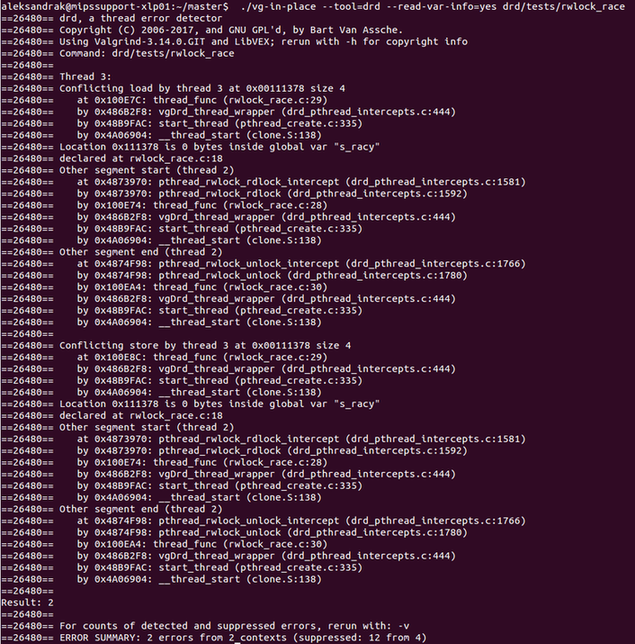
\includegraphics[scale=0.75]{slika20.png}
\end{center}
\caption{Пример детекције трке за подацима}
\label{fig:drd-data-race}
\end{figure}

\indent \textit{DRD} исписује поруку сваки пут када открије да је дошло до трке за подацима у програму. Треба имати у виду пар следећих ствари приликом тумачења исписа који нам алат \textit{DRD} даје. Прво, \textit{DRD} додељује свакој нити јединствени број \textit{ID}. Бројеви који се додељују нитима крећу од један и никада се не користи исти број за више нити. Друго, термин сегмент се односи на секвенцу узастопних операција чувања, читања и синхронизације које се извршавају у једној нити. Сегмент увек почиње и завршава се операцијом синхорнизације. Анализа трке за подацима се извршава између два сегмента уместо између појединачних операција читања и чувања података, искључиво због учинка. На крају, увек постоје два приступа меморији приликом трке за подацима. \textit{DRD} штампа извештај о сваком приступу меморији које је довело до трке за подацима.

\indent На слици \ref{fig:drd-data-race} је дат испис алата \textit{DRD} када пронађе да је дошло до трке за подацима у програму~\cite{drdRef}.



\paragraph{Алгоритам детекциjе приступа променљивој без синхронизације у оквиру алата \textit{Helgrind}} \mbox{}\\

\begin{figure}[h!]
\begin{center}
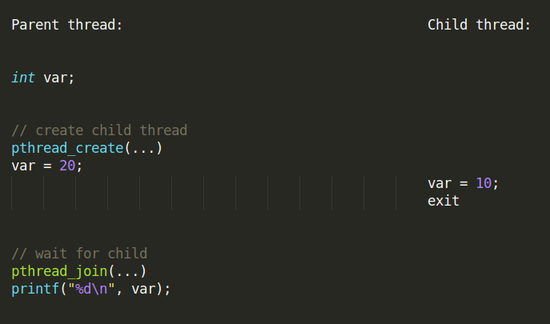
\includegraphics[scale=0.75]{slika16.png}
\end{center}
\caption{"Десило се пре" релација}
\label{fig:dspPrincip}
\end{figure}


\indent Алгоритам за детекцију приступа промељивој без синхронизације имплементира "десило се пре" релацију (енгл. \textit{"happens-before" relation}). У наставку је дат пример који објашњава "десило се пре" релацију \ref{fig:dspPrincip}.

\indent Нит родитељ креира нит дете. Затим обе мењају вредност промељиве \textit{var}, а затим нит родитеља чека да нит детета изврши своју функцију. Овај програм није добро написан јер не можемо са сигурношћу да знамо која је вредност промљиве \textit{var} приликом штамања исте. Ако је нит родитеља бржа од нити дете, онда ће бити штампана вредност 10, у супротном ће бити 20. Брзина извршавања нити родитељ и дете је нешто на шта програмер нема утицаја. Решење овог проблема је у закључавању промељиве \textit{var}. На пример, можемо да пошаљемо поруку из нити родитељ након што она промени вредност промељиве \textit{var}, а нит дете неће променити вредност променљиве \textit{var} док не добије поруку. На овај начин смо сигурни  да ће програм исписати вредност 10. Размена порука креира "десило се пре" зависност између две доделе вредност: \textit{var = 20;} се догађа пре \textit{var = 10;}. Такође, сада више немамо приступ променљивој без синхронизације. Није обавезно да шаљемо поруку из нити родитељ. Можемо послати поруку из нити дете након што она изврши своју доделу. На овај начин смо сигурни да ће се исписати вредност 20.

\indent Алат \textit{Helgrind} ради на истом овом принципу. Он прати сваки приступ меморијској локацији. Ако се локација, у овом примеру \textit{var}, приступа из две нити, \textit{Helgrind} проверава да ли су ти приступи повезани са "десило се пре" везом. Ако нису, алат пријављује грешку о приступу променљивој без синхронизације.

\indent Ако је приступ дељеној променљивој из две или више програмерске нити повезан са "десило се пре" релацијом, значи да постоји синхорнизациони ланац између програмских нити које обезбеђује да се сам приступ одвија по тачно одређеном редоследу, без обзира на стварне стопе напретка појединачних нити.

\indent Стандардне примитиве нити креирају "десило се пре" релацију:
\begin{itemize}
  \item Ако је мутекс откључан од стране нити $T_1$, а касније или одмах закључан од стране нити $T_2$, онда се приступ меморији у функцији $T_2$ дешава пре него што нит  $T_2$ откључа мутекс да би приступила меморији.
  \item Иста идеја се односи и на \textit{reader-writer} закључавање променљивих.
  \item Ако је кондициона промељива сигнализирана у фукнцији нити $T_1$ и ако друга нит $T_2$ чека на тај сигнал, да би наставила са радом, онда се меморијски приступ у $T_1$ дешава пре сигнализације, док нит $T_2$ врши приступ меморији након што изађе из стања чекања на сигнал који шаље нит $T_1$.
  \item Ако нит $T_2$ наставља са извршавањем након што нит $T_1$ ослободи семафор, онда кажемо да постоји "десило се пре" релација између програмских нити $T_1$ и $T_2$.
\end{itemize}

\indent \textit{Helgrind} пресреће све горе наведене догађаје и креира граф који представља све "десило се пре" релације у програму. Такође, он прати све приступе меморији у програму. Ако постоји приступ некој меморијској локацији у програму од стране две нити и \textit{Helgrind} не може да нађе путању кроз граф од једног приступа до другог, генерише податак о грешци у програму који анализира.

\indent \textit{Helgrind} не проверава да ли постоји приступ меморијској локацији без синхорнизације уколико се сви приступи тој локацији односе на читање садржаја те локације. Два приступа су у "десило се пре" релацији, иако постији призвољно дугачак ланац синхронизације догађаја између та два приступа. Ако нит $T_1$ приступа локацији $M$, затим сигнализира нит $T_2$, која касније сигнализира нит $T_3$ која приступа локацији $M$, кажемо да су ова два приступа између нити $T_1$ и $T_3$ у "десило се пре" релацији, иако између њих не постоји директна веза.

\indent \textit{Helgrind} алгоритам за детекцију приступа меморији без синхорнизације прикупљене информације приказује у форми приказаној на слици \ref{fig:helgrind}. 

\indent На слици \ref{fig:helgrind} можемо да приметимо да \textit{Helgrind} најпре исписује податке где су нити које узрокују грешку направљене. Главни података о грешци почиње са \textit{"Possibal data race during read"}. Затим се исписује адреса где се несинхрони приступ меморији дешава, као и величина меморије којој се приступа. У наставку \textit{Helgrind} исписује где друга нит приступа истој локацији. На крају, \textit{Helgrind} покренут са опцијом \textit{-\--read-var-inof=yes} исписује и само име променљиве којој се приступа, као и где у програму је та променљива декларисана~\cite{helgrindRef}.

\subsection{Задржавање катанаца}

\indent Приликом рада нити може доћи до појаве задржавања катанца, при којој једна нит не може да ради због блокирања других нити. Дешава се да нит мора да чека да мутекс или синхорнизациони \textit{reader-write} објекат буду откључани од стране друге нити. Оваква појава је непожељна у вишенитним системима, алат \textit{DRD} открива овај тип проблема.

\indent Задржавање катанаца ствара кашњења, која би требало да буду што је могуће краћа. Опције \textit{-\--exclusive-threshold=<n>} и \textit{-\--shared-threshold=<n>} омогућавају да \textit{DRD} открије претерано задржавање катанца, тако што ће пријавити свако задржавање катанца које је дуже од задатог прага~\cite{drdRef}.

\indent Алат \textit{Helgrind} не открива овакав тип грешака.


\section{Callgrind}
\label{section_callgrind}

\begin{figure}[h!]
\begin{center}
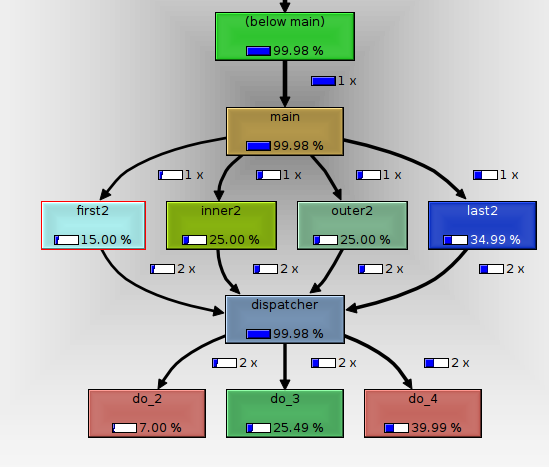
\includegraphics[scale=0.75]{slika18.png}
\end{center}
\caption{Пример визуелизације функција}
\label{fig:callgrind}
\end{figure}

\indent \textit{Callgrind} је алат који генерише листу позива функција корисничког програма у виду графа. У основним подешавањима сакупљени подаци састоје се од броја извршених инструкција, њихов однос са линијом у извршном коду, однос позиваоц/позван између функција, као и број таквих позива. Додатна подешавања омогућавају анализирање кода током изршавања. 

\indent Подаци који се анализирају се записују у фајл након завршетка рада програма и алата. Подржане команде су:

\begin{description}
	\item[\textit{callgrind\_annotate}] - на основу генерисаног фајла приказује листу функција. Пример визуелизације листе функција приказан је на слици \ref{fig:callgrind}. За графичку визуелизацију препоручују се додатни алати (\textit{KCashegrind}), који олакшава навигацију уколико \textit{Callgrind} направи велику количину података.
	\item[\textit{callgrind\_control}] - ова команда омогућава интераквину контролу и надгледање програма приликом извршавања. Могу се добити информације о стању на стеку, може се такође у сваком тренутку генерисати профил~\cite{callgrindRef}.
\end{description}


\indent Алат \textit{Cachgrind} сакупља податке, односно броји догађаје који се дешавају директно у једној функцији. Овај механизам сакупљања података се назива ексклузивним.

\indent Алат \textit{Callgrind} проширује ову фукнционалност тако што пропагира цену функције до њених граница. На пример, ако фукнција \textit{foo} позива фукнцију \textit{bar}, цена функције \textit{bar} се додаје фукнцији \textit{foo}. Када се овај механизам примени на целу функцију, добија се слика такозваних инклузивних позива, где цена сваке функције укључује и цене свих фукнција које она позива, директно или индиректно.

\indent Захваљујући графу позива, може да се одреди, почевши од \textit{main} функције, која фукнција има највећу цену позива. Позиваоц/позван цена је изузетно корисна за профилисање фукнција које имају више позива из разних функција, и где имамо прилику за оптимизацију нашег програма мењајући к\^{о}д у функцији која је позиваоц, тачније редуковањем броја позива.

\indent Могућност детектовања свих позива функција, као и зависност инструкција алата  \textit{Callgrind} зависи од платформе на којој се извршава. Овај алат најбоље ради на \textit{x86} и \textit{amd64}, али нажалост не даје најтачније резултате на следећим платформама \textit{PowerPc}, \textit{ARM} и \textit{MIPS}. Разлог томе је што код наведених платформи не постоји експлицитан позив или инструкција у скупу инструкција, па  \textit{Callgrind} мора да се ослања на хеуристике да би детектовао позиве или инструкције~\cite{callgrindRef}.


\section{Massif}
\label{section_massif}

\begin{figure}[h!]
\begin{center}
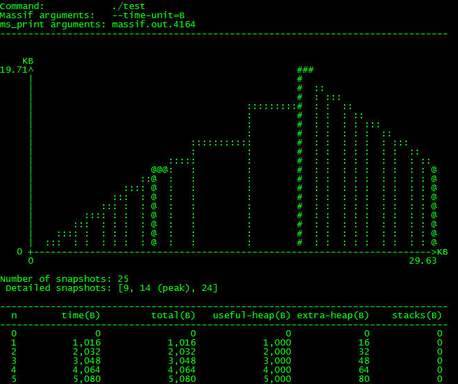
\includegraphics[scale=0.75]{slika19.png}
\end{center}
\caption{Приказ оптерећења хипа коришћењем \textit{Massif} алата}
\label{fig:massif}
\end{figure}

\indent \textit{Massif} је алат за анализу хип меморије корисничког програма. Обухвата, како меморију којој корисник може да приступи, тако и меморију која се користи за помоћне концепте као што су \textit{book-keeping} бајтова и простор за поравнање. Може да израчуна величину стек меморије програма, али ова опција није подразумевана, већ мора експлицитно да се наведе.

\indent Анализа програмског хипа, на модерним рачунарима који користе виртуалну меморију, доноси предност у виду убрзавања програма, јер мањи програми имају бољу искоришћеност кеша и избегавају страничење. Код програма који захтевају велику количину меморије, добра искоришћеност хипа смањује шансу за изгладљивањем простора за размену (енг. \textit{swap space}) корисничке машине.

\indent Постоје одређени сценарији цурења меморије који не спадају у класичне, и такве пропусте не могу детектовати алати као што је \textit{Memcheck}. Ово се дешава зато што меморија није заправо изгубљена, показивач на њу и даље постоји, али она се више не користи. Програми са оваквим типом цурења меморије доводе до непотребног коришћења одређене количине меморије током свог извршавања. \textit{Massif} помаже у откривању баш оваквих цурења меморије.

\indent \textit{Massif} не даје само информацију о томе колико хип меморије се користи, већ и детаљне информације које упућују на то који део програма је одговоран за алоцирање те меморије~\cite{massifdRef}.

\subsection{Коришћење \textit{Massif}-а}


\indent Програм који се извршава под алатом \textit{Massif} ради веома споро. Након завршетка рада, све статистике су исписане у фајл. Подразумевани фајл у који се пише је \textit{massif.out.<pid>}, где \textit{<pid>} представља ID процеса. Може се променити фајл у коме ће се исписивати командом \textit{-\--massif-out-file}.

\indent Да би информације које је \textit{Massif} сакупио могли да видимо у читљивом формату, користимо \textit{ms\_print}. Ако имамо фајл \textit{massif.out.1234}: 


\begin{center}
 ms\_print massif.out.1234
\end{center}

\indent \textit{ms\_print} прозводи граф који показује на трошење меморије током извршавања програма, као и детаљне информације о различитим тачкама програма које су одговорне о алокацији меморији. Коришћење различитих скрипти за презентацију резултата је намерно, јер одваја сакупљање података од презентације, као и да је могуће додати нов начин приказа података у сваком тренутку.

\indent На слици \ref{fig:massif} приказан је пример излаза из алата \textit{Massif}. Величина графа може бити промењена коришћењем \textit{ms\_print} опција \textit{-\--x} и \textit{-\--y}. Свака вертикала представља пресек стања искоришћености меморије у одређеном тренутку времена. Текст на дну слике \ref{fig:massif} показује да смо имали 25 пресека. \textit{Massif} почиње тако што одради пресек за сваку алокацију и деалокацију хипа, али ако се програм извршава дуже \textit{Massif} све ређе врши пресеке. У случају сложених програма, који се извршавају дуже \textit{Massif} не чува почетне пресеке када достигне максималну вредност пресека. Подразумевана количина пресека коју алат \textit{Massif} чува је 100, ово се може променити коришћењем опције \textit{-\--max-snapshots}. Ово значи да је одговарајући број пресека стања сачуван у сваком тренутку рада програма.

\indent Одређени пресеци су детаљније обрађени. Обрађени пресеци су представљени у графу знаком '@'. На дну слике \ref{fig:massif} је наглашено да постоје три стања која су детаљније обрађена (стање 9, 14 и 24). Подразумевано је да се свако десето стање обрађује детаљније, али и ово се може променити опцијом \textit{-\--detailed-freq}.

\indent Детањније обрађени пресеци могу бити представљени и знаком '\#', али у том случају значи да је искоришћеност меморије у том тренутку била највећа. Овакав пресека мора да се појави барем једном у графу. На слици \ref{fig:massif} се види да је такав пресек, пресек број 14.

\indent Утврђивање који од пресека је пресек са најискоришћенијом меморијом није увек тачан. Разлог томе је да \textit{Massif} узима у обзир само пресеке код којих се десила деалокација, овим се избегава обрађивање многих непотребних пресека, али значи да ако програм никада не деалоцира меморију, неће бити обрађених пресека са најискоришћенијом меморијом. Још један разлог јесте да обрађивање пресека са најискоришћенијом меморијом одузима доста времана. Због тога \textit{Massif} чува само она стања чија величина износи 1\% од величине пресека где је искоришћеност меморије била највећа~\cite{massifdRef}.

\subsection{Мерење целокупне меморије}


\indent Треба нагласити да алат \textit{Massif} мери само хип меморију, односно меморију која је алоцирана \textit{malloc}, \textit{calloc}, \textit{realloc}, \textit{memalign}, \textit{new}, \textit{new[]} и пар других сличних функција. Ово значи да \textit{Massif} не мери меморију која је алоцирана системским позивима као што су \textit{mmap}, \textit{mremap} и \textit{brk}. Такође, у програму могу да постоје системски позиви за алоцирање меморије, \textit{Massif} неће узети у обзир ту меморију током анализе програма.

\indent Уколико нам је од великог значаја да се узме у обзир сва алоцирана меморија у нашем програму, потребно је укључити опцију \textit{-\--pages-as-heap=yes}. Укључивањем ове опције, \textit{Massif} неће профајлирати хип меморију, већ странице у меморији~\cite{massifdRef}.


\chapter{Имплементација конвенције \textit{FPXX}}
\label{chp:fpxx}

\indent Сама структура \textit{Valgrind} језгра се може поделити на два дела \textit{VEX} и \textit{coregrind}. У \textit{VEX} делу су имплеметиране инструкције за сваку од архитектура коју \textit{Valgrind} подржава, односно овај део је одговоран за дисасембрирање и асемблирање. У \textit{VEX} делу најбитнија функција за дисасемблирање је \textit{disInstr\_MIPS}, ова функција је различита за сваку архитектуру и њено име је у складу са сваком архитектуром. У овој функцији се врши дисаемблирање свих инструкција у \textit{IR}. Приликом асемблирања избор инструкција врши се рекурзивним обиласком стабла инструкција у дубину, где су за обилазак зависно од типа вредности израза коришћене следеће функције: \textit{iselWordExpr\_R} користи се за целобројне вредности,  \textit{iselInt64Expr} за 64-битне на 32-битном \textit{MIPS}-u, \textit{iselDblExpr} за 64-битне вредности са покретним зарезом на 32-битним системима и \textit{iselFltExpr} за вредности са покрентим зарезом. Обилажење се почиње функцијом \textit{iselSB\_MIPS} којој се прослеђује сам исказ. Све ове функције смештене су у фајлу 
\textit{VEX/priv/\-host\_mips\_isel.c}. У фајлу \textit{VEX/priv/guest\_mips\_helpers.c} садржане су помоћне функције које се умећу у \textit{Valgrind}-ов к\^{о}д ради иницијализације и израчунавања флегова који постављају инструкције које раде са бројевима у покретном зарезу. У фајловима \textit{coregrind/m\_syswrap/syswrap-mips32-linux.c} и \textit{coregrind/m\_syswrap\-/syswrap-mips64-linux.c} је одређено пресретање системских позива за 32-битну и 64-битну архитектуру \textit{MIPS}.


\indent У \textit{coregrind} је смештен управљачки део \textit{Valgrind}-а, имплементација системских позива и сигнала. Најбитнији део овде јесте фајл  \textit{coregrind/m\_scheduler/\-scheduler.c}. У овом фајлу се организује извршавање програма који се пушта кроз \textit{Valgrind} и покреће \textit{Valgrind}-ове системе за управљање системским позивима и сигналима. Пре покретања програма кроз функције у фајлу \textit{coregrind/\-m\_scheduler/scheduler.c} потребно је утврдити могућности система, што се ради у фајлу \textit{m\_machine.c}, као и постављање система за управљање меморијом програма који се извршава. У фајлу \textit{coregrind/m\_ume/elf.c} се налазе функције које читају и обрађују заглавље учитаног програма. 

\indent У оквиру рада су решавана два проблема. Први проблем је био да се омогући превођење самог алата \textit{Valgrind} са опцијом \textit{-mfpxx}, док је други проблем био да се омогући да се програми преведени са опцијом \textit{-mfpxx} коректно извршавају кроз \textit{Valgrind}.

\indent Да би могле да се виде измене које су прихваћене потребно је имати цео к\^{о}д алата \textit{Valgrind}. Преузимање кода врши се покретањем следеће команде у терминалу:

\begin{center}
git clone git://sourceware.org/git/valgrind.git
\end{center}

Након тога треба се лоцирати у директоријуму алата. У наставку ће бити дате команде које је потребно извршити из терминала и директоријума у коме се налази код алата \textit{Valgrind}.

\section{Превођење алата \textit{Valgrind} са опцијом \textit{-mfpxx}}

\indent Да би омогућили превођење алата \textit{Valgrind} са опцијом \textit{-mfpxx}, било је потребно прилагодити асемблерске делове \textit{Valgrind}-а тако да буду у складу са конвенцијом \textit{FPXX}. На слици \ref{fig:asm} је приказана промена асемблерског дела алата \textit{Valgrind}, односно уклањање из коришћења регистара са непарним индексом. Инструкција \textit{mtc1} замењена је инструкцом \textit{ldc1} пошто она ради са 64-битним вредностима, односно смешта 64-битну вредност у \textit{FP} регистар. Ова измена је имплементира у \textit{VEX/priv/guest\_mips\_helpers.c}. Као што се види на слици промењена су два макроа која се позивају из функције \textit{mips\_dirtyhelper\_\-calculate\_FCSR\_fp32}. Ова измена се може видети покретањем следеће команде у терминалу

\begin{center}
git show 2746f7e70b2737b0744592409564463a9203c5f0
\end{center}

\begin{figure}[h!]
\begin{center}
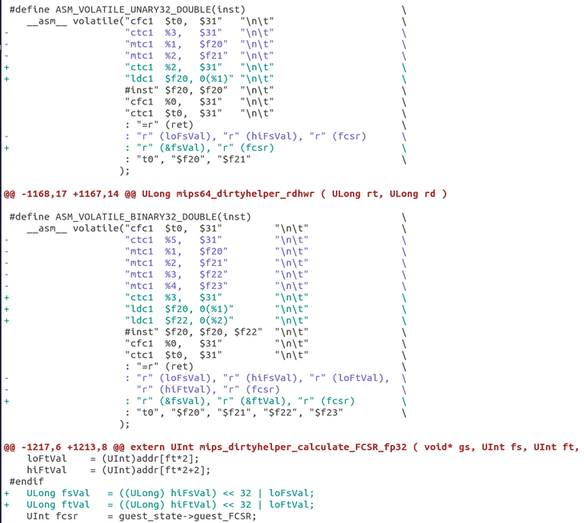
\includegraphics[scale=0.75]{slika26.png}
\end{center}
\caption{Прилагођавање асемблерских делова алата \textit{Valgrind}}
\label{fig:asm}
\end{figure}

\indent Имплементацијом ове измене, више није познато у ком режиму ће се \textit{Valgrind} извршавати, што повлачи додатне измене кода алата \textit{Valgrind}, које су описане у наставку.

\section{Детектовање режима у којем ради алат \textit{Valgrind}}

\indent Након омогућавања превођења алата \textit{Valgrind} са опцијом \textit{-mfpxx}, следећи задатак је био детектовање режима у ком се \textit{Valgrind} извршава. Детекција самог режима имплементирана је у \textit{coregrind} делу, тачније у фајлу \textit{coregrind/m\_mach\-ine.c} у функцији \textit{machine\_get\_hwcaps}. У овој функцији се одређују карактеристике система, као што је начин уписа у меморију. Овде је одређена и детекција \textit{FP} режима у ком алат \textit{Valgrind} треба да ради. Претходна имплементација, која је и уклоњена, није узимала у обзир могућност више \textit{FP} режима.
 На слици \ref{fig:detekcija} је приказана имплементација саме детекције.

\begin{figure}[h!]
\begin{center}
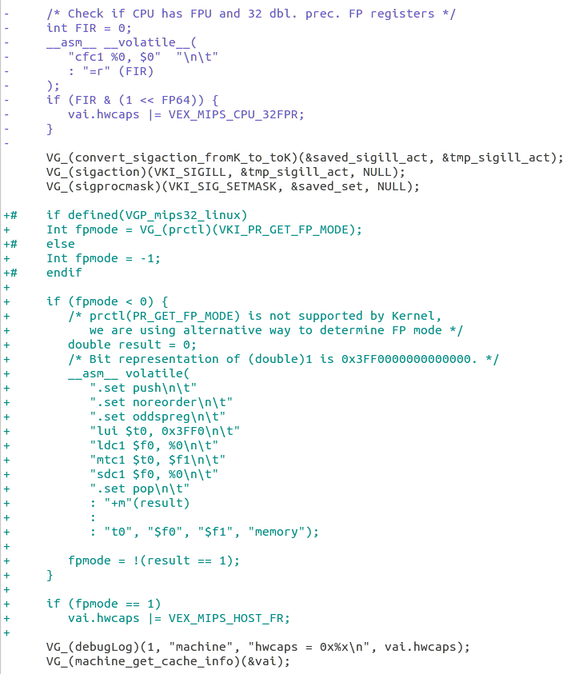
\includegraphics[scale=0.75]{slika27.png}
\end{center}
\caption{Детектовање режима}
\label{fig:detekcija}
\end{figure}

\indent Овде се прво врши провера да ли језгро подржава \textit{PR\_GET\_FP\_MODE} и \textit{PR\_SET\_FP\_MODE} опције . Уколико их не подржава извршава се асемблерски код. Инструкција \textit{sdc1} се извршава другачије у зависности од режима и помоћу ње ми добијамо информацију у ком режиму треба да ради сам алат \textit{Valgrind}.

Ова измена се може видети покретањем следеће команде у терминалу

\begin{center}
git show 030cea68c804abc61facd95e894a1c8b2418904f
\end{center}

\section{Одређивање режима у којем програм почиње са радом}


\indent \textit{Valgrind} као виртуална машина ради у једном \textit{FPU} режиму, ако је преведен са опцијом  \textit{-mfpxx} онда ће радити у режиму које језгро одреди. С друге, стране он емулира јединицу за операције са покретним зарезом, с тога може да емулира другачији режим рада. Због тога је потребно имплементирати алгоритам за избор \textit{FPU} режима као што је то урађено у језгру. У фајлу \textit{coregrind/m\_ume/elf.c} имплементиране су следеће функције \textit{arch\_elf\_pt\_proc()} и \textit{arch\_check\_elf()}. За имплементацију ових функција као референца се може користити  функције из језгра, тачније функције у фајлу 
linux/arch/mips/kernel/elf.c. Функција \textit{arch\_elf\_pt\_proc()} проверава заглавље учитаног програма да провери исправност и/или подобност у односу на систем на ком се извршава. Функција \textit{arch\_\-check\_elf()} одређује у ком режиму ће радити програм који се пушта кроз \textit{Valgrind}. На слици \ref{fig:fre} дат је део функције \textit{arch\_check\_elf()} у ком се одређује режим рада. 

\begin{figure}[h!]
\begin{center}
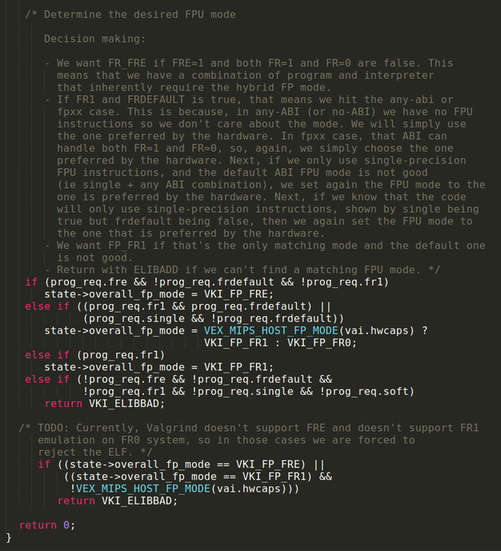
\includegraphics[scale=0.75]{slika29.png}
\end{center}
\caption{Одређивање режима у којем програм почиње са радом}
\label{fig:fre}
\end{figure}

Ова измена се може видети покретањем следеће команде у терминалу

\begin{center}
git show 030cea68c804abc61facd95e894a1c8b2418904f
\end{center}

\section{Пресретање системског позива prtcl()}

\begin{figure}[h!]
\begin{center}
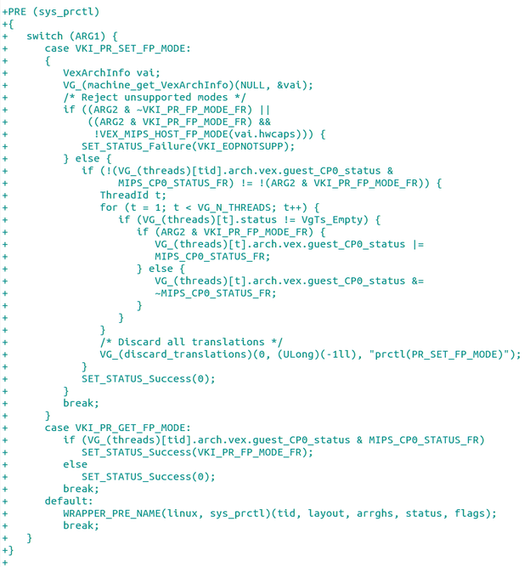
\includegraphics[scale=0.75]{slika28.png}
\end{center}
\caption{Пресретање системског позива \textit{prctl()}}
\label{fig:prctl}
\end{figure}

\indent У одређеним ситуацијама \textit{Valgrind} мора да пресретне системске позиве и сам их обрађује. Потреба за таквим случајем јавља се и приликом имплементације овог решења. Пресретање системског позива \textit{prctl()} у \textit{Valgrind}-у је било неопходно да би подршка за режим \textit{FPXX} била потупуна. Пресретање системског позива \textit{prctl()} је одрађена у фајловима \textit{coregrind/m\_syswrap/syswrap-mips32-linux.c} и \textit{coregrind/m\_syswrap/syswrap-mips64-linux.c}. Овај системски позив је обавијен макроом \textit{PRE}, што значи да алат \textit{Valgrind} неће допустити да \textit{prctl()} оде до самог језгра, већ ће он сам одрадити све што је потребно. Имплементација пресретања систесмког позива \textit{prctl()} дата је на слици \ref{fig:prctl}. На слици се види да се одрађена имплементација флегова \textit{PR\_GET\_FP\-\_MODE} и \textit{PR\_SET\_FP\-\_MODE}. Сви флегови који су дефинисани у самом коду језгра, дефинисани су и у алату \textit{Valgrind}, једина разлика је у префиксу \textit{VKI}.

\indent Приликом имплементације флега \textit{PR\_SET\_FP\-\_MODE}, врши се пролазак кроз све активне нити и мења се режим у ком оне раде. Функција \textit{SET\-\_STATUS\_Success(0)} спречава системски позив да оде до самог језгра и изврши се, већ се овде зауставља.

Ова измена се може видети покретањем следеће команде у терминалу

\begin{center}
git show 030cea68c804abc61facd95e894a1c8b2418904f
\end{center}

\section{Тестирање}

\indent У почетним фазама развоја тестирано је само правилно препознавање \textit{FP} режима у којем ради програм. Ово је рађено помоћу једноставног програма који је превођен на различите начине. Касније, како је развој привођен крају, тестирање је вршено помоћу теста који током свог извршавања мења режим рада. Овај тест је сада један од тестова којим се свакодневно проверава исправност рада алата \textit{Valgrind}. Путања до теста, уколико се налазимо у самом директоријуму \textit{Valgrind} алата, је none/tests/mips32/change\_fp\_mode.c. На слици \ref{fig:changefp} је приказан део теста где се детектује и мења режим рада. Као што може да се види, на два начина се детектује режим, један је помоћу асемблерског кода, док је други помоћу системског позива \textit{prctl()} и флага \textit{PR\_GET\_FP\_MODE}. Врши се провара променљивих у којима су сачуване вредности режима, да ли имају исту вредност. Након тога се мења режим рада помоћу системског позива \textit{prctl()} и флага \textit{PR\_SET\_FP\_MODE} и опет се врши детектција режима. Током извршавања тестова алат \textit{Valgrind} користи скрипту која врши проверу да ли је излаз који даје тест исти као очекивани, односно као излаз програма када ради без \textit{Valgrind} алата. Сваки тест има фајл у којем се налази излаз без посредства \textit{Valgrind} алата. Ако се ова два излаза поклапају, значи да је тест прошао и да алат \textit{Valgrind} исправно ради.

\begin{figure}[h!]
\begin{center}
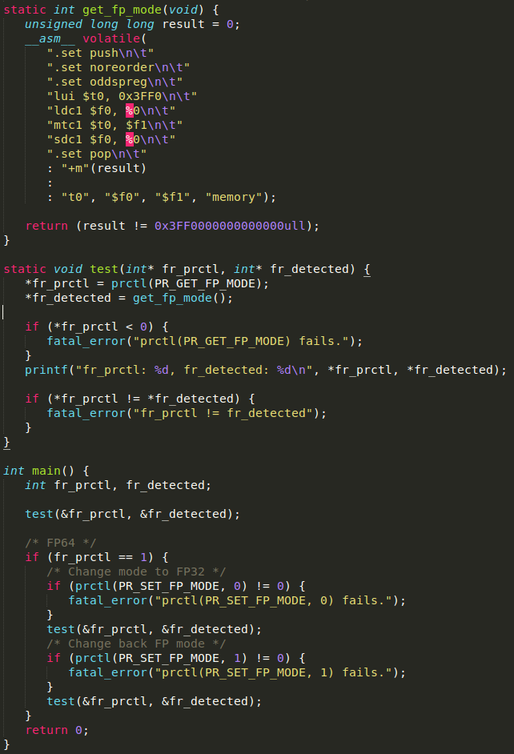
\includegraphics[scale=0.75]{slika30.png}
\end{center}
\caption{Тест \textit{change\_fp\_mode.c}}
\label{fig:changefp}
\end{figure}

\chapter{Закључак}

\indent Откривање грешака попут цурења меморије и утркивања приликом приступа податку од стране више нити у великим системи може бити веома напорно, дуготрајно па и немогуће у неким случајевима. Анализом кода посредством \textit{Valgrind} алата може се уштедети драгоцено време. Помоћу \textit{Valgrind} алата могу се открити грешке које не утичу на исправност рада програма, али знатно утичу на перформансе програма, уколико се не отркију. Грешке које могу да се пронађу су многобројне. Алат \textit{Memcheck} открива меморијске грешке које су често и најтеже за детектовање. Неки од проблема које може да отркије јесу коришћење неицијализованих вредности или неипсравно ослобађање хип меморије. Алат \textit{Cachgrind} симулира и прати приступ брзој меморији машине на којој се програм  извршава. Алати \textit{Helgrind} и \textit{DRD} су одлични за детековање и уклањање грешака које се јављају приликом рада са нитима. Алат \textit{Massif} анализира хип меморију корисничког програма и алат \textit{Callgrind} врши анализу графа позива функција.

\indent Циљ овог рада је био упознавање са алатом \textit{Valgrind} и додавање подршке за конвенцију \textit{FPXX}. Како је ова конвенција специфична за архитектуру \textit{MIPS}, на почетку рада дата је кратка историја и осврт на специфичности ове архитектуре. Описани су регистри који су битни у архитектури \textit{MIPS}, а мало већи акценат је стављен на регистре за рад са бројевима у покрентом зарезу. Архитектура \textit{MIPS} користи два формата ових регистара, регистре са једноструком и двоструком прецизношћу.

\indent У овом раду је описана конвенција \textit{FPXX} као и њена имплементација у алату \textit{Valgrind}. Једна од првих карактеристика је била забрана коришћења регистара са непарним индексом, па је то био један од првих задатака током имплементације. Обрађен је и системски позив \textit{prctl()}, коме је посвећена пажња приликом анализе, па и имплементације. Након завршетка имплементације, алат \textit{Valgrind} има много већи спектар употребе и анализе програма.

\indent Као могући правац даљег рада, планира се додавање имплементације \textit{FRЕ=1} режима. Наиме, овај режим је саставни део конвенције \textit{FPXX} при чему алат \textit{Valgrind} тренутно нема подршку за овај режим. Да би се додао овај режим, потребно је додавање подршке за \textit{MIPS R6} скуп инструкција.


% ------------------------------------------------------------------------------

% ------------------------------------------------------------------------------
% Literatura
% ------------------------------------------------------------------------------
\literatura

% ==============================================================================
% Završni deo teze i prilozi
\backmatter
% ==============================================================================

% ------------------------------------------------------------------------------
% Biografija kandidata
% ------------------------------------------------------------------------------

\begin{biografija}
\textbf{Александра Караџић} (\emph{Приштина, 11. јануар 1992.}) Рођена сам у Приштини. Завршила сам Гимназију у Лесковцу, природно математички смер, 2010. године и исте године уписала Математички факултет у Београду. 2015. године сам завршила основне студије Математичког факултета и исте уписала мастер студије. Положила сам све испите са мастер студија у септембру 2017. године. Од маја 2015. године па до сада радим као инжењер у \textit{RT-RK}. Пројекат на ком сам започела свој рад у фирми \textit{RT-RK} је пројекат на ком и даље радим, а то је одржавање и развој алата \textit{Valgrind} за \textit{MIPS} архитектуру.
\end{biografija}

\end{document}